%----------------------------------------------------------------------------
\chapter{Részletes megvalósítás}
\label{sec:Details}
%----------------------------------------------------------------------------

Ebben a fejezetben a korábban röviden bemutatott építőelemekről adok egy részletesebb leírást.  
Bemutatom, hogy az én projektemben milyen megoldásokat valósítottam meg a használatukkal.  
Ahol van értelme, diagramokon keresztül mutatom be a működésüket, ami látványos, azt képekkel is illusztrálom.  
Több kódrészlet is szerepelni fog a fejezetben, amelyek célja a kód működésének jobb megértése.  

\section{Compose}
\label{sec:Compose}

A Composeról korábban már adtam egy átfogó leírást a \refstruc{sec:JetpackCompose}-ban. Most ebben a részben részletesebben bemutatom az alapelemeket, használatát és a következő képernyőket.  

\subsection{Compose alapelvek, használata valós környezetben}

Mivel a Compose egy deklaratív UI kit, ezért összefoglalnám a legfontosabb részeit.  
A UI elemeket nem lehet direktben példányosítani és kódból később elérni, illetve ezen a referencián keresztül módosítani a tulajdonságaikat.  
Minden egyes elem egy függvényhívást jelent, az állapotát és tulajdonságait pedig ezen belül lehet szabályozni és beállítani egyéb objektumokon és state-eken keresztül.  
Ezeket az állapotokat általában nem a Composable függvényen belül tároljuk, hanem egy ViewModelben, mivel az tartósabb. (\refstruc{fig:ViewModel})  
Egy figyelt állapot hatására meghívódik a recomposition, azaz a függvény újra meghívódik, és frissíti a UI állapotát.  
Az általános elv az, hogy egy Composable függvény nagy betűvel kezdődik, és attól lesz egy függvény Composable, hogy elé helyezzük a @Composable annotációt.  

Mi is az a recomposition?  
Röviden, valamilyen állapotváltozást követő újra kirajzolódás.  
Gyakran valamilyen felhasználói interakció váltja ki (gomb megnyomása, görgetés), de a ViewModelből is jöhet ez a változás (megérkezik a kezdeti adat, folyamatosan frissülő információk jönnek), illetve okozhatja egy animáció is.  

A Compose használatának van 5 fontos alapszabálya, amelyek betartásával nemcsak helyes, de gyors és dinamikusan frissülő képernyőket tudunk egyszerűen létrehozni.  
\begin{enumerate}
    \item A Composable függvények bármilyen sorrendben végrehajthatók.  
    \item A Composable függvények párhuzamosan hajthatók végre.  
    \item A Recomposition kihagyja a lehető legtöbb Composable függvényt és lambdát.  
    \item A Recomposition optimista, és leállítható menet közben.  
    \item Egy Composable függvény nagyon gyakran is futhat/ismétlődhet, olyan gyakran is, mint egy animáció minden képkockája.  
\end{enumerate}

Pontosan mit is jelentenek ezek a szabályok?
Az 1. és 2. pont alapján következik, hogy minden Composable függvény önálló legyen, nem függhet egy másik Composable függvénytől sem.  
Továbbá fontos, hogy ha ugyanazon state-et változtatják, akkor az ne fusson le minden recomposition során. Ha ezt nem tartjuk be, akkor folyamatosan újra kirajzolódik a képernyő, és lefagy az eszköz.  
A 3. pont értelmezése, hogy csak a szükséges részek renderelődnek újra, ezzel gyorsítva a folyamatot. Így, amennyiben több függvényt is meghívunk egy másikon belül, csak azok fognak újra kirajzolódni, amelyek függnek a változott állapottól.  
Előfordulhat, hogy mindent szeretnénk újra frissíteni, vagy több függvényt, amelyek nem függnek tőle. Ehhez használhatunk az állapottól függő LaunchedEffect-et, vagy átadhatjuk az állapotot ezeknek a függvényeknek is, és ott csinálhatunk velük egy egyszerű és gyors műveletet.  
A 4. és 5. pont összefügg: ha új állapot érkezik, és nem fejeződött be a recomposition, akkor elölről kezdi a folyamatot. Ne itt hajtsunk végre hosszú műveletet (HTTP kérések indítása), mert ez felesleges overhead-et jelent, mivel senki nem állítja le az aszinkron hívást, és nem tud hova visszaérkezni az adat, így feleslegesen használtuk az erőforrásokat mindkét oldalon.  
Ne állítsunk be egy olyan értéket sem itt, amire szükségünk lehet később, mivel nem biztos, hogy eljut a futás addig, vagy lehet, hogy a következő másodpercben már felül lett írva mással.

Az alábbi kódrészletben bemutatom, hogy milyen részekből tevődik össze egy Composable függvény.
\begin{lstlisting}[caption={Composable függvény részei.}, label={lst:ComposableParts}, language=Kotlin]
@Composable     // A kötelező annotáció
fun ExamEditResultScreen(   // Függvényparaméterek
    navigateBack: () -> Unit,       // Egy lambda függvény fejléce
    viewModel: ExamEditViewModel,   // ViewModel átadása paraméterként
    modifier: Modifier = Modifier   // Modifier amivel a kinézetet lehet testre szabdni.
) {
    val coroutineScope = rememberCoroutineScope()           // Coroutine scope lekérése, így lambda függvényben használható, mivel annak a törzse nem Composable függvény.
    var showNotify by remember { mutableStateOf(false) }    // Statek amit el lehet tárolni a Composable függvényben mivel ezen kívül nincs használva.
    var notifyMessage by remember { mutableStateOf("") }    // Statek amit el lehet tárolni a Composable függvényben mivel ezen kívül nincs használva.
    if (showNotify) { Notify(notifyMessage); showNotify = false} // Állapottól függő megjelenítés
    Scaffold(   // Beépített Composable elem amivel egy általános Android nézetet könnyen létre lehet hozni.
        topBar = { TopAppBarContent(stringResource(Res.string.exam_edit), navigateBack) },  // Itt egy topBart lehet könnyen megadni.
    ){innerPadding ->   // Ez a belső része a képernyőnek, a fő része az alkalmazásnak.
        ExamEntryBody(      // Egy másik Composable elem meghívása, ami a megjelenésért felel.
            examUiState = viewModel.examUiState,           // Szüksége van viewModelben lévő statere
            onExamValueChange = viewModel::updateUiState,  // Nevesített függvényt így lehet átadni egy lambda függvénynek
            onSaveClick = {     // Lambda függvényt helyben is megadhatunk
                coroutineScope.launch { // Itt látható egy példa a trailing lambda használatára
                    if(viewModel.updateExam()){ navigateBack() }    // If-else szerkezet is nyugodtan használhatunk. Siker esetén visszanavigál
                    else{   // Egyébként a sikertelenséget közli a felhasználóval
                        showNotify = true
                        notifyMessage =  "Exam with this name already exists"
                    }
                }
            },
            modifier = modifier.padding(innerPadding))}}
\end{lstlisting}

\subsection{Alkalmazás bemutatása képernyőképekkel}

Ebben az alfejezetben bemutatom az elkészült képernyőket és a hozzájuk tartozó érdekes részeket, megoldásokat.

\subsubsection{A fő képernyők}

A két alkalmazás típusra más-más a felhasználói igény.
Androidon, ahol általában egy álló képernyő van (\refstruc{fig:MainScreen} jobb oldal), és a telefont a jobb alsó sarokban fogjuk meg, nem esik kézre a fent bekapcsolható menü (bár oldalra húzással is előhozható). 
Asztali alkalmazás esetén viszont jobban mutat ez a megoldás, és egy nagyobb képernyőn a kiválasztott funkció képernyője meg tud jelenni (\refstruc{fig:MainScreen} bal oldal és \refstruc{fig:OpenMenu}).
Későbbiekben a navigálásban is segít, így könnyebb képernyőt váltani. A fenti vissza gomb használata kevésbé kényelmes, mint Androidon, egy gyors mozdulat a telefon alján, ahol a kezünkkel tartjuk azt.

Ennek megfelelően a MainScreen függvény a közös kódban egy expect függvény, és így minden platformra az oda illő actual implementációt tudjuk megírni és alkalmazni.
Végül más megoldást választottam a navigációhoz, így az asztali alkalmazásnál a szintén expect/actual NavHost létrehozásakor nem kapnak értéket a függvények.
\begin{lstlisting}[caption={Expect Főképernyő.}, label={lst:ExpectMainScreen}, language=Kotlin]
@Composable
expect fun MainScreen(
    navigateToTopicList: () -> Unit = {},
    navigateToPointList: () -> Unit = {},
    navigateToTrueFalseQuestionList: () -> Unit = {},
    navigateToMultipleChoiceQuestionList: () -> Unit = {},
    navigateToExamList: () -> Unit = {},
    navigateToExportExamList: () -> Unit = {},
    navigateToSubmission: () -> Unit = {},
    onSignOut: () -> Unit = {},
)
\end{lstlisting}
\begin{figure}[!ht]
    \centering
    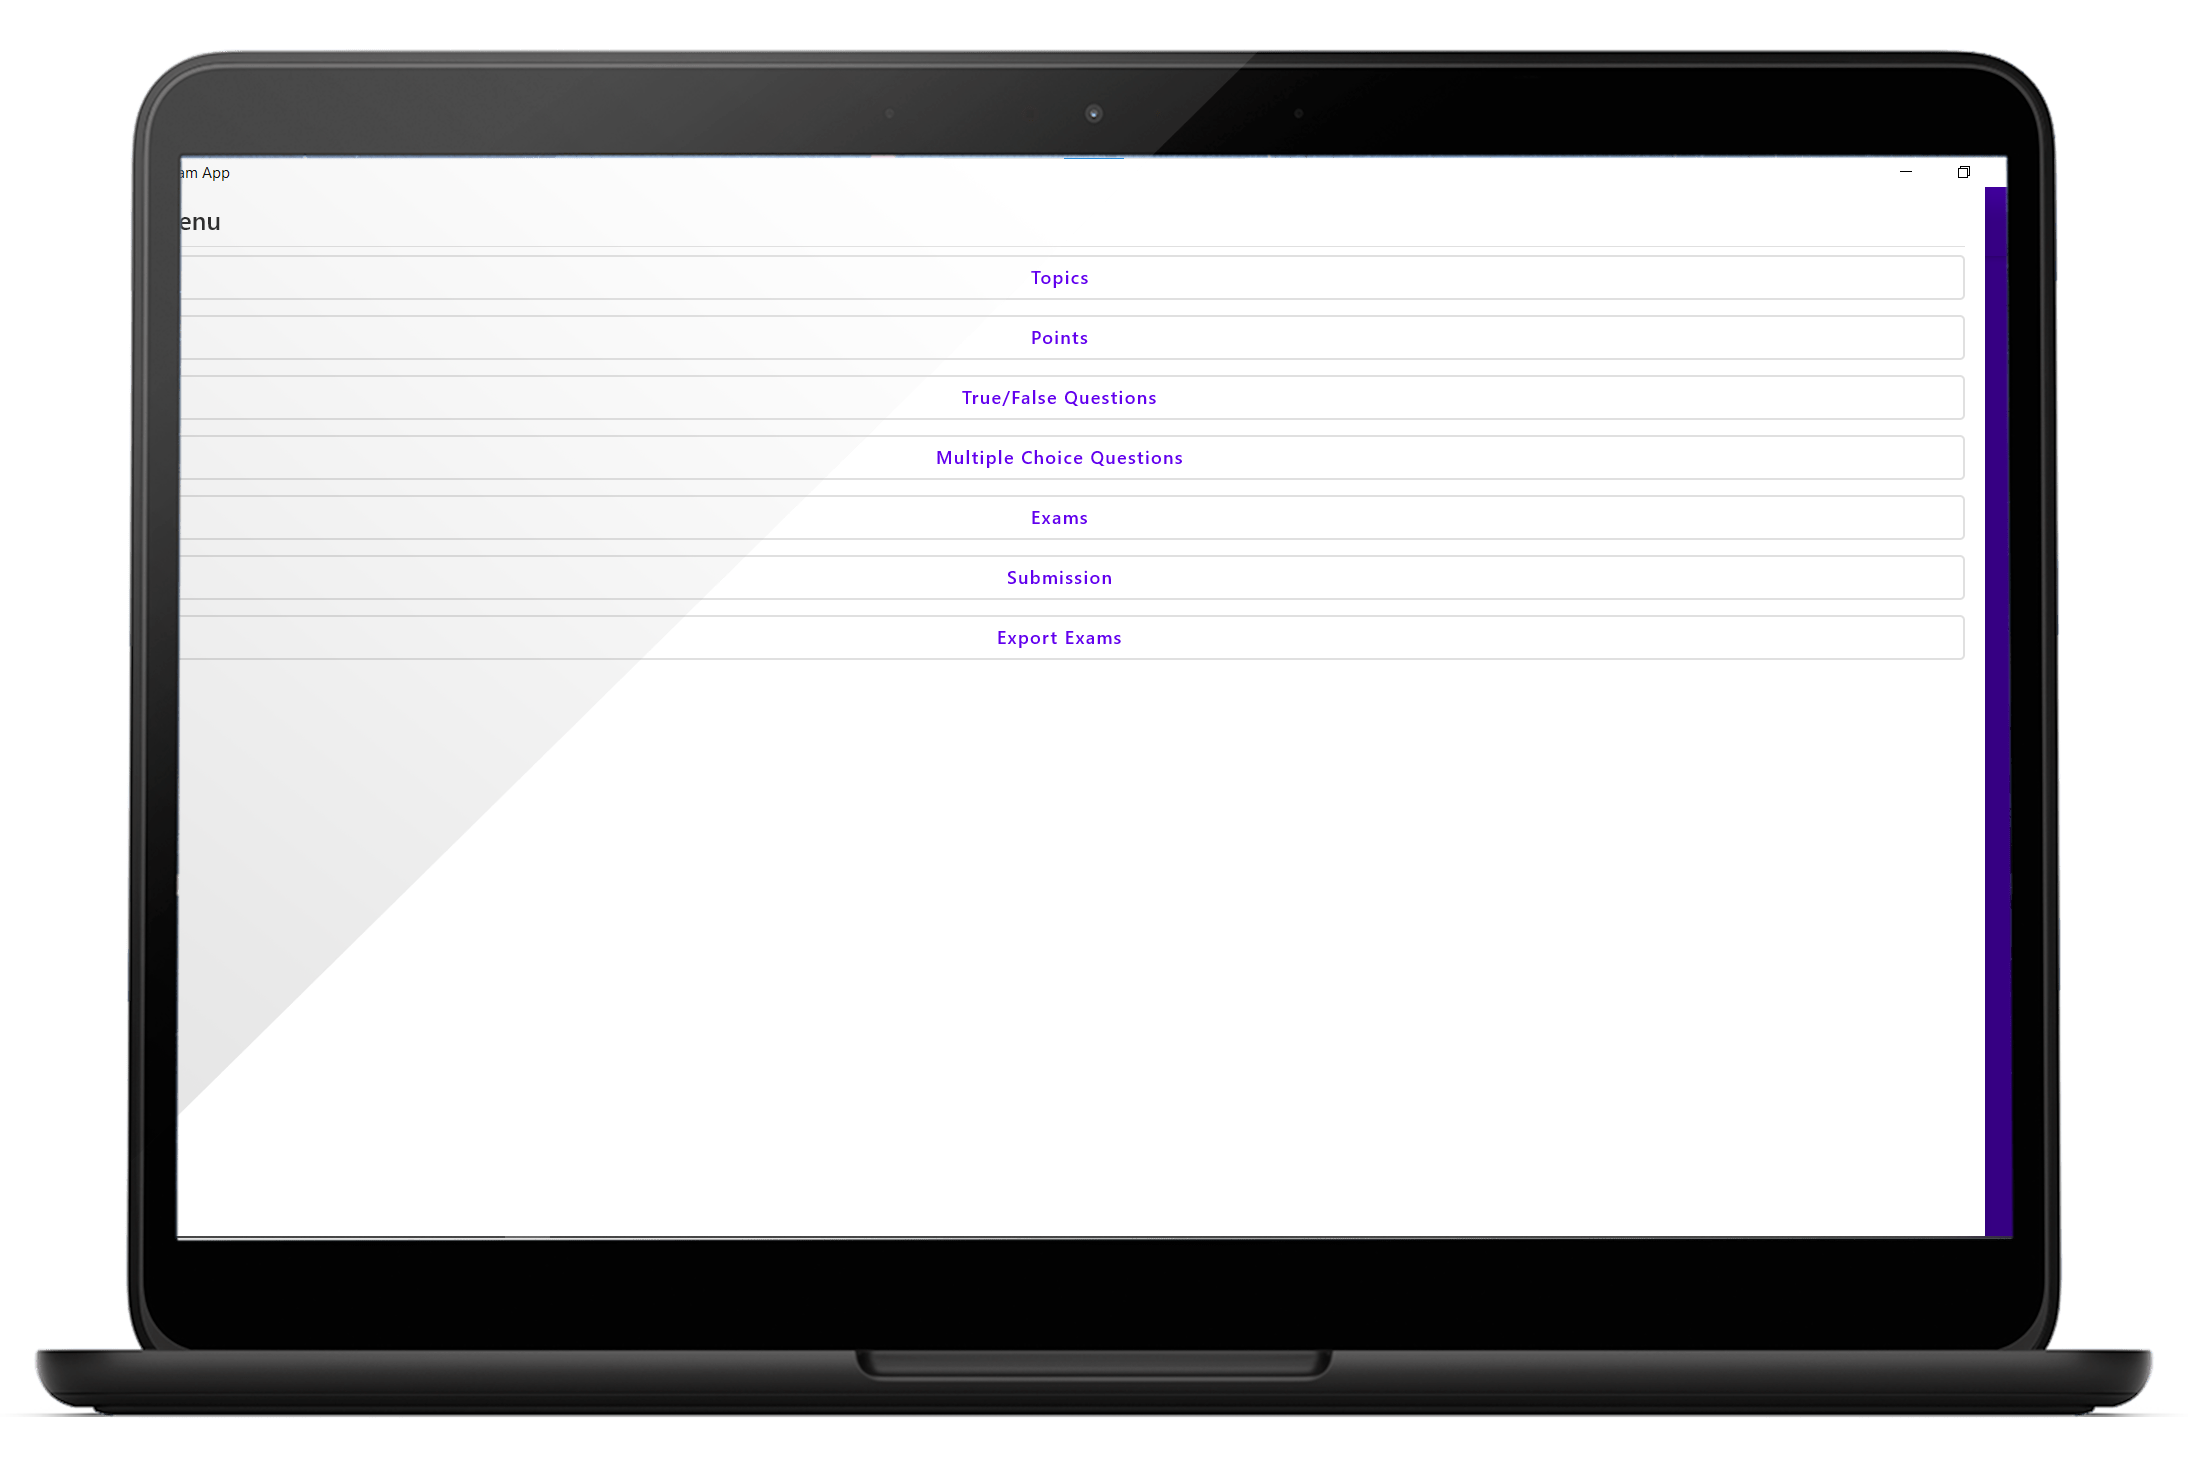
\includegraphics[width=0.5\textwidth, keepaspectratio]{figures/MainScreen_Desktop2_framed.png}
    \caption{Kinyitott menüsáv kinézete az asztali alkalmazáson}
    \label{fig:OpenMenu}
\end{figure}

\begin{figure}[!ht]
    \centering
    \begin{tabular}{cc}
        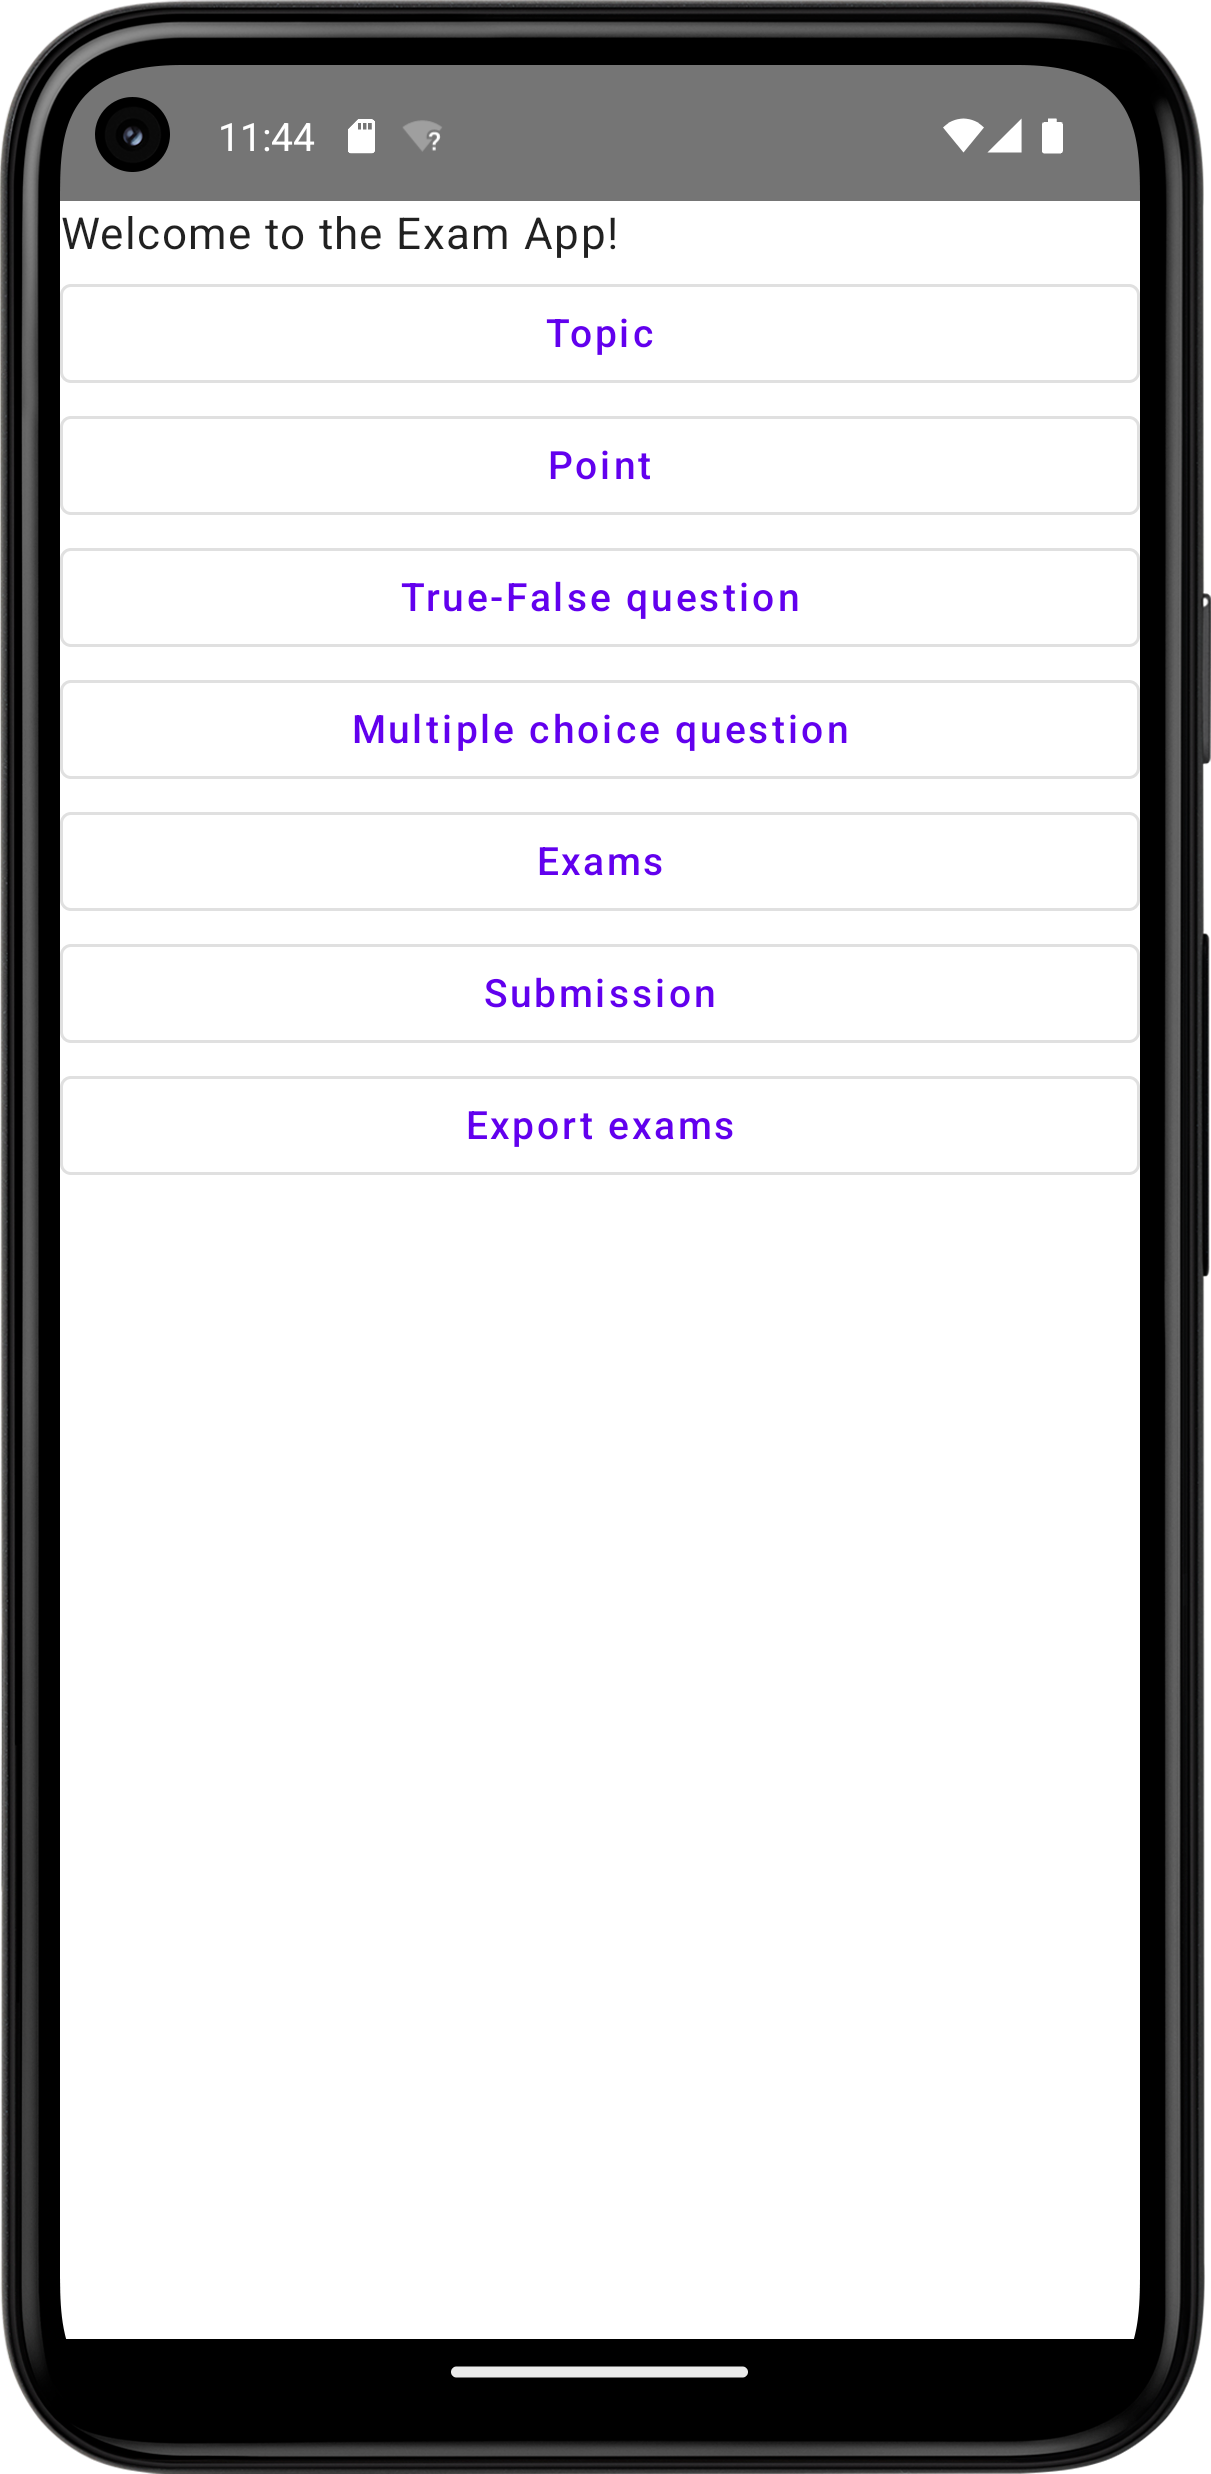
\includegraphics[width=0.3\textwidth, keepaspectratio]{figures/MainScreen_Android.png} & 
        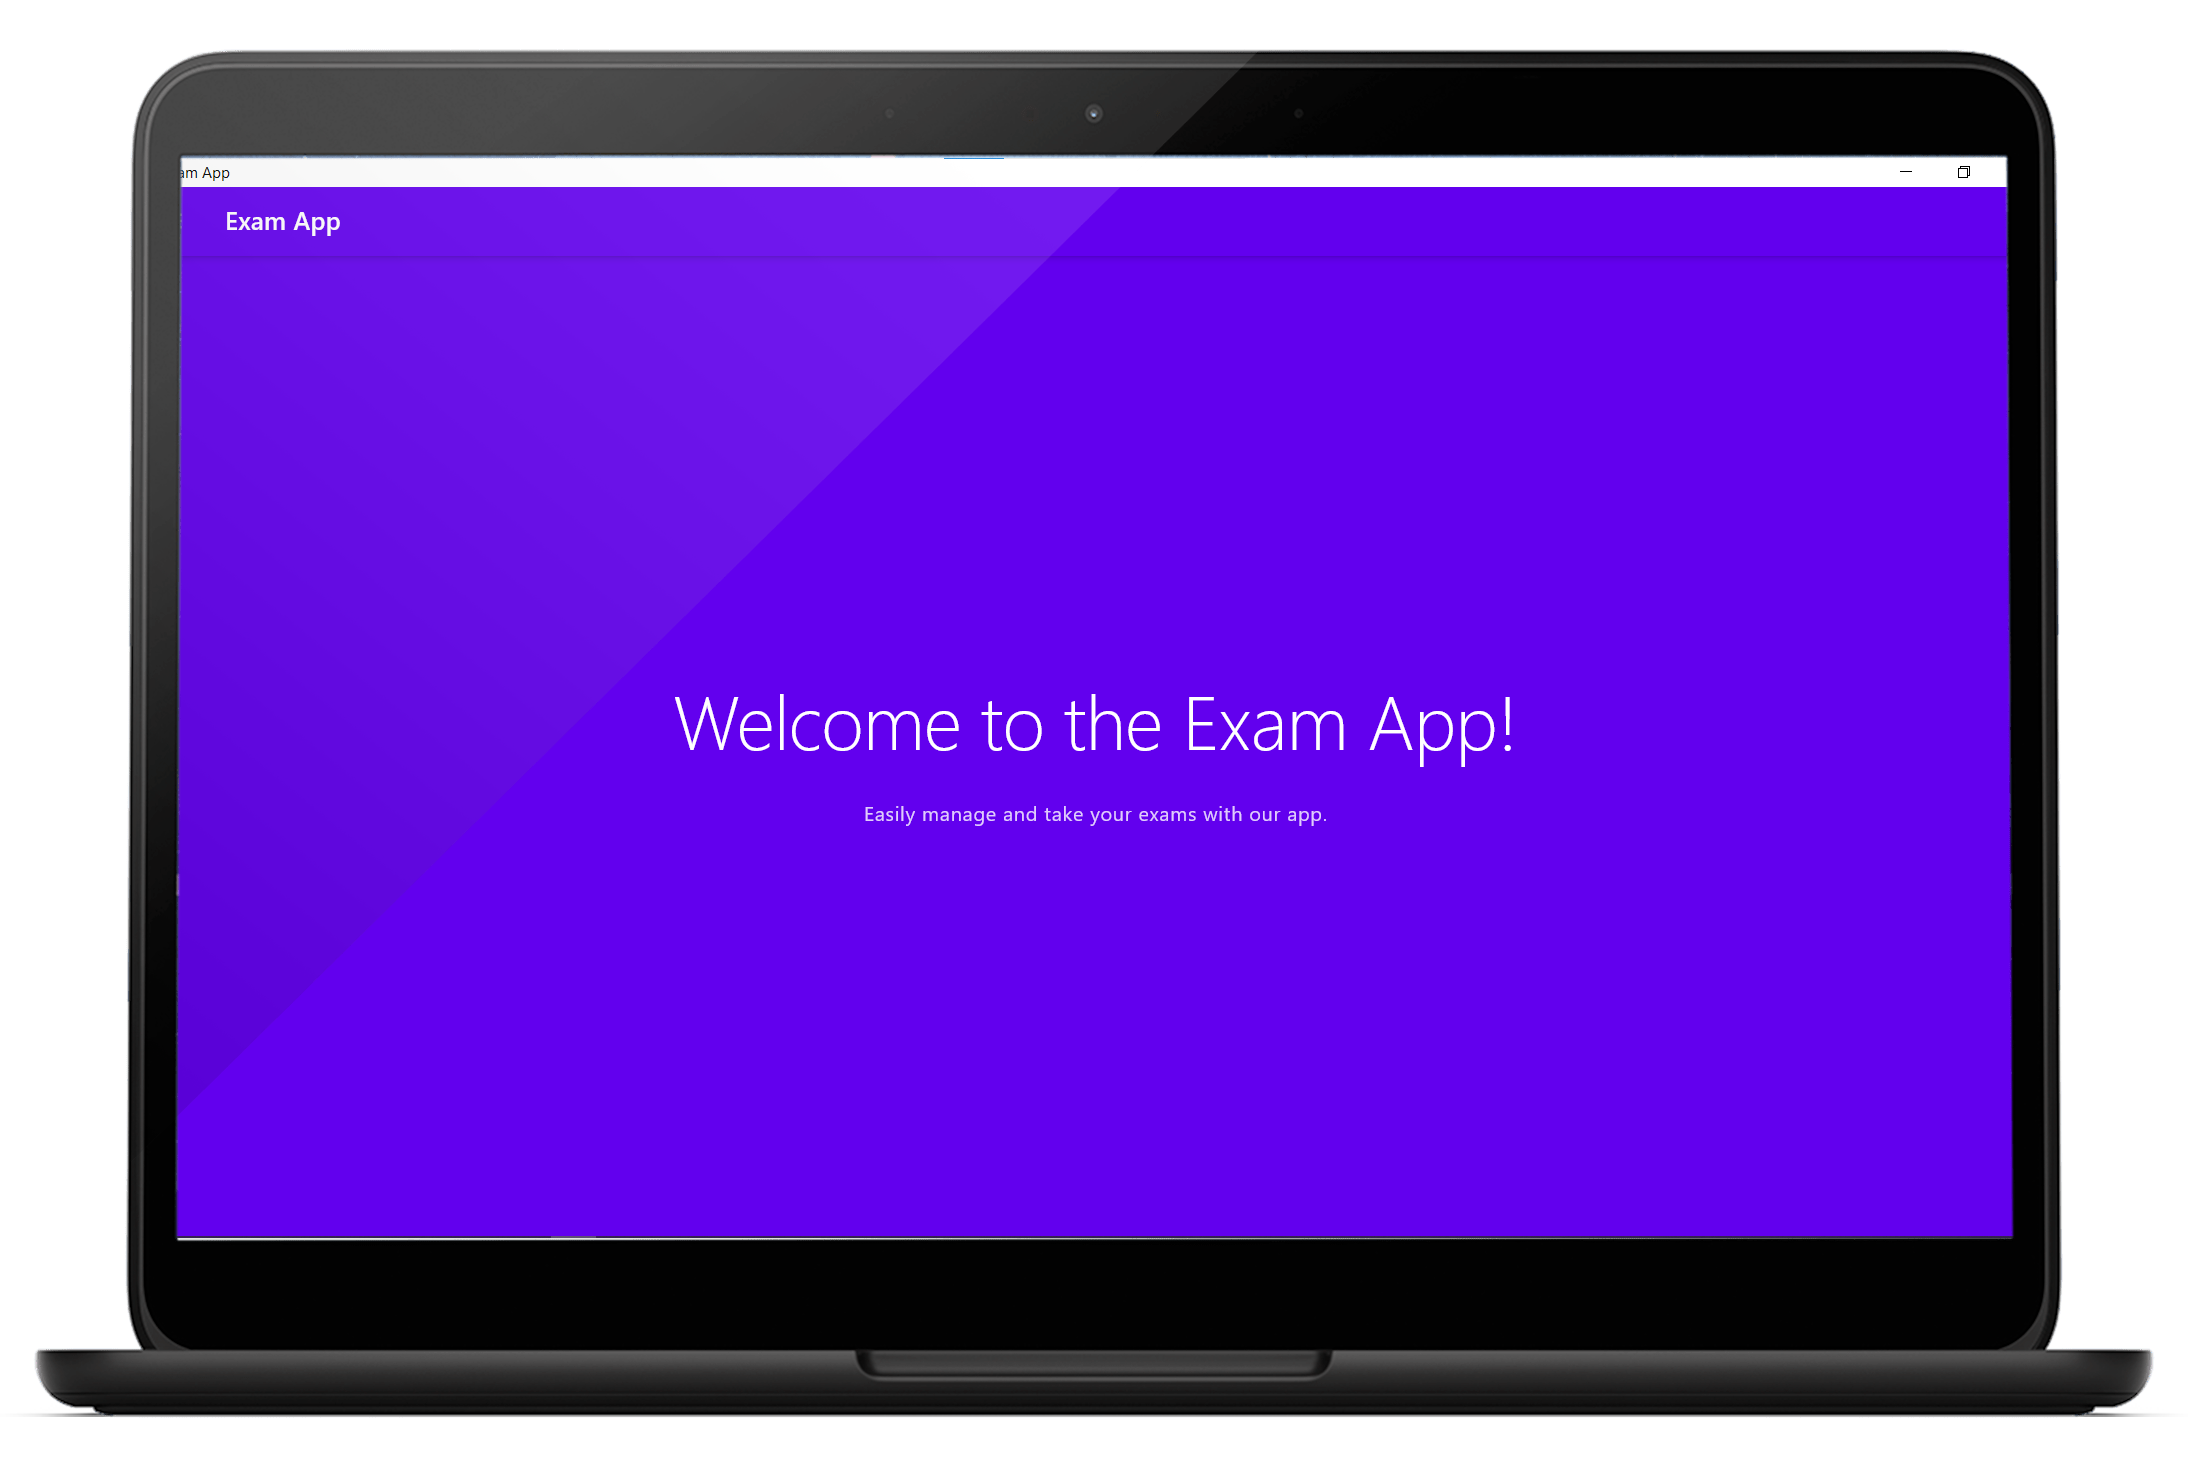
\includegraphics[width=0.5\textwidth, keepaspectratio]{figures/MainScreen_Desktop1_framed.png}
    \end{tabular}
    \caption{A fő képernyő Android és asztali alkalmazáson}
    \label{fig:MainScreen}
\end{figure}


\pagebreak

\subsubsection{Elemek listázása}

Az elemek felsorolásáért egy LazyColumn felelős. (\ref{lst:ListScreen}.~kódrészlet)
Ez egy előre létrehozott, beépített Composable függvény.
Több hasznos tulajdonsággal rendelkezik. Alapértelmezett módon görgethetővé válik, ha több elem van benne, mint amennyi kifér egy képernyőre. (\refstruc{fig:ListScreen})
Alkalmas nagyon sok, akár végtelen elem megjelenítésére, bár ehhez szükség van az adatok ügyes betöltésére is. 
Mindig csak annyi elemet renderel ki, amennyi éppen szükséges, látszódik. Előtte és utána van egy kis tartalék puffer, így görgetés esetén nem kell várni az új adatok betöltésére.
Az elemek testre is szabhatók benne, tökéletes alkalmazási területe lehet egy chat alkalmazás, ahol az elemeket az üzenet küldője alapján lehet színezni.

\begin{lstlisting}[caption={Listázó képernyő.}, label={lst:ListScreen}, language=Kotlin, float]
@Composable
fun MultipleChoiceQuestionListResultScreen( ...
) {
    Scaffold(
        topBar = { TopAppBarContent(stringResource(Res.string.mc_question_list), navigateBack) },
        floatingActionButton = {
            FloatingActionButton(
                onClick = { addNewQuestion() }, ...
            ) {Icon(Icons.Filled.Add, contentDescription = "Add") } }
    ) { padding ->
        LazyColumn(
            contentPadding = padding, ...) {
            if (questions.isEmpty()) {  item { Box(modifier = Modifier ...) { Text(...) } }
            } else {
                items(questions) { question ->
                    TextButton( onClick = { navigateToMultipleChoiceQuestionDetails(question.uuid) }, ... ) { Text(text = question.name, ...) 
}}}}}}
\end{lstlisting}

Ezen a képernyőn is a Scaffold megoldást választottam, így kényelmesen elfér egy navigációs sáv és egy Floating Action Button az új elemek felvételéhez.
Ezeken túl több korábban is bemutatott elem megjelenik ebben a kódrészletben is.
Ahogy látszik az \ref{lst:ListScreen}.~kódrészletben is, attól függően lehet elemeket beállítani, hogy milyen feltételhez kötjük az elemek megjelenítését.

\begin{figure}[!ht]
    \centering
    \begin{tabular}{cc}
        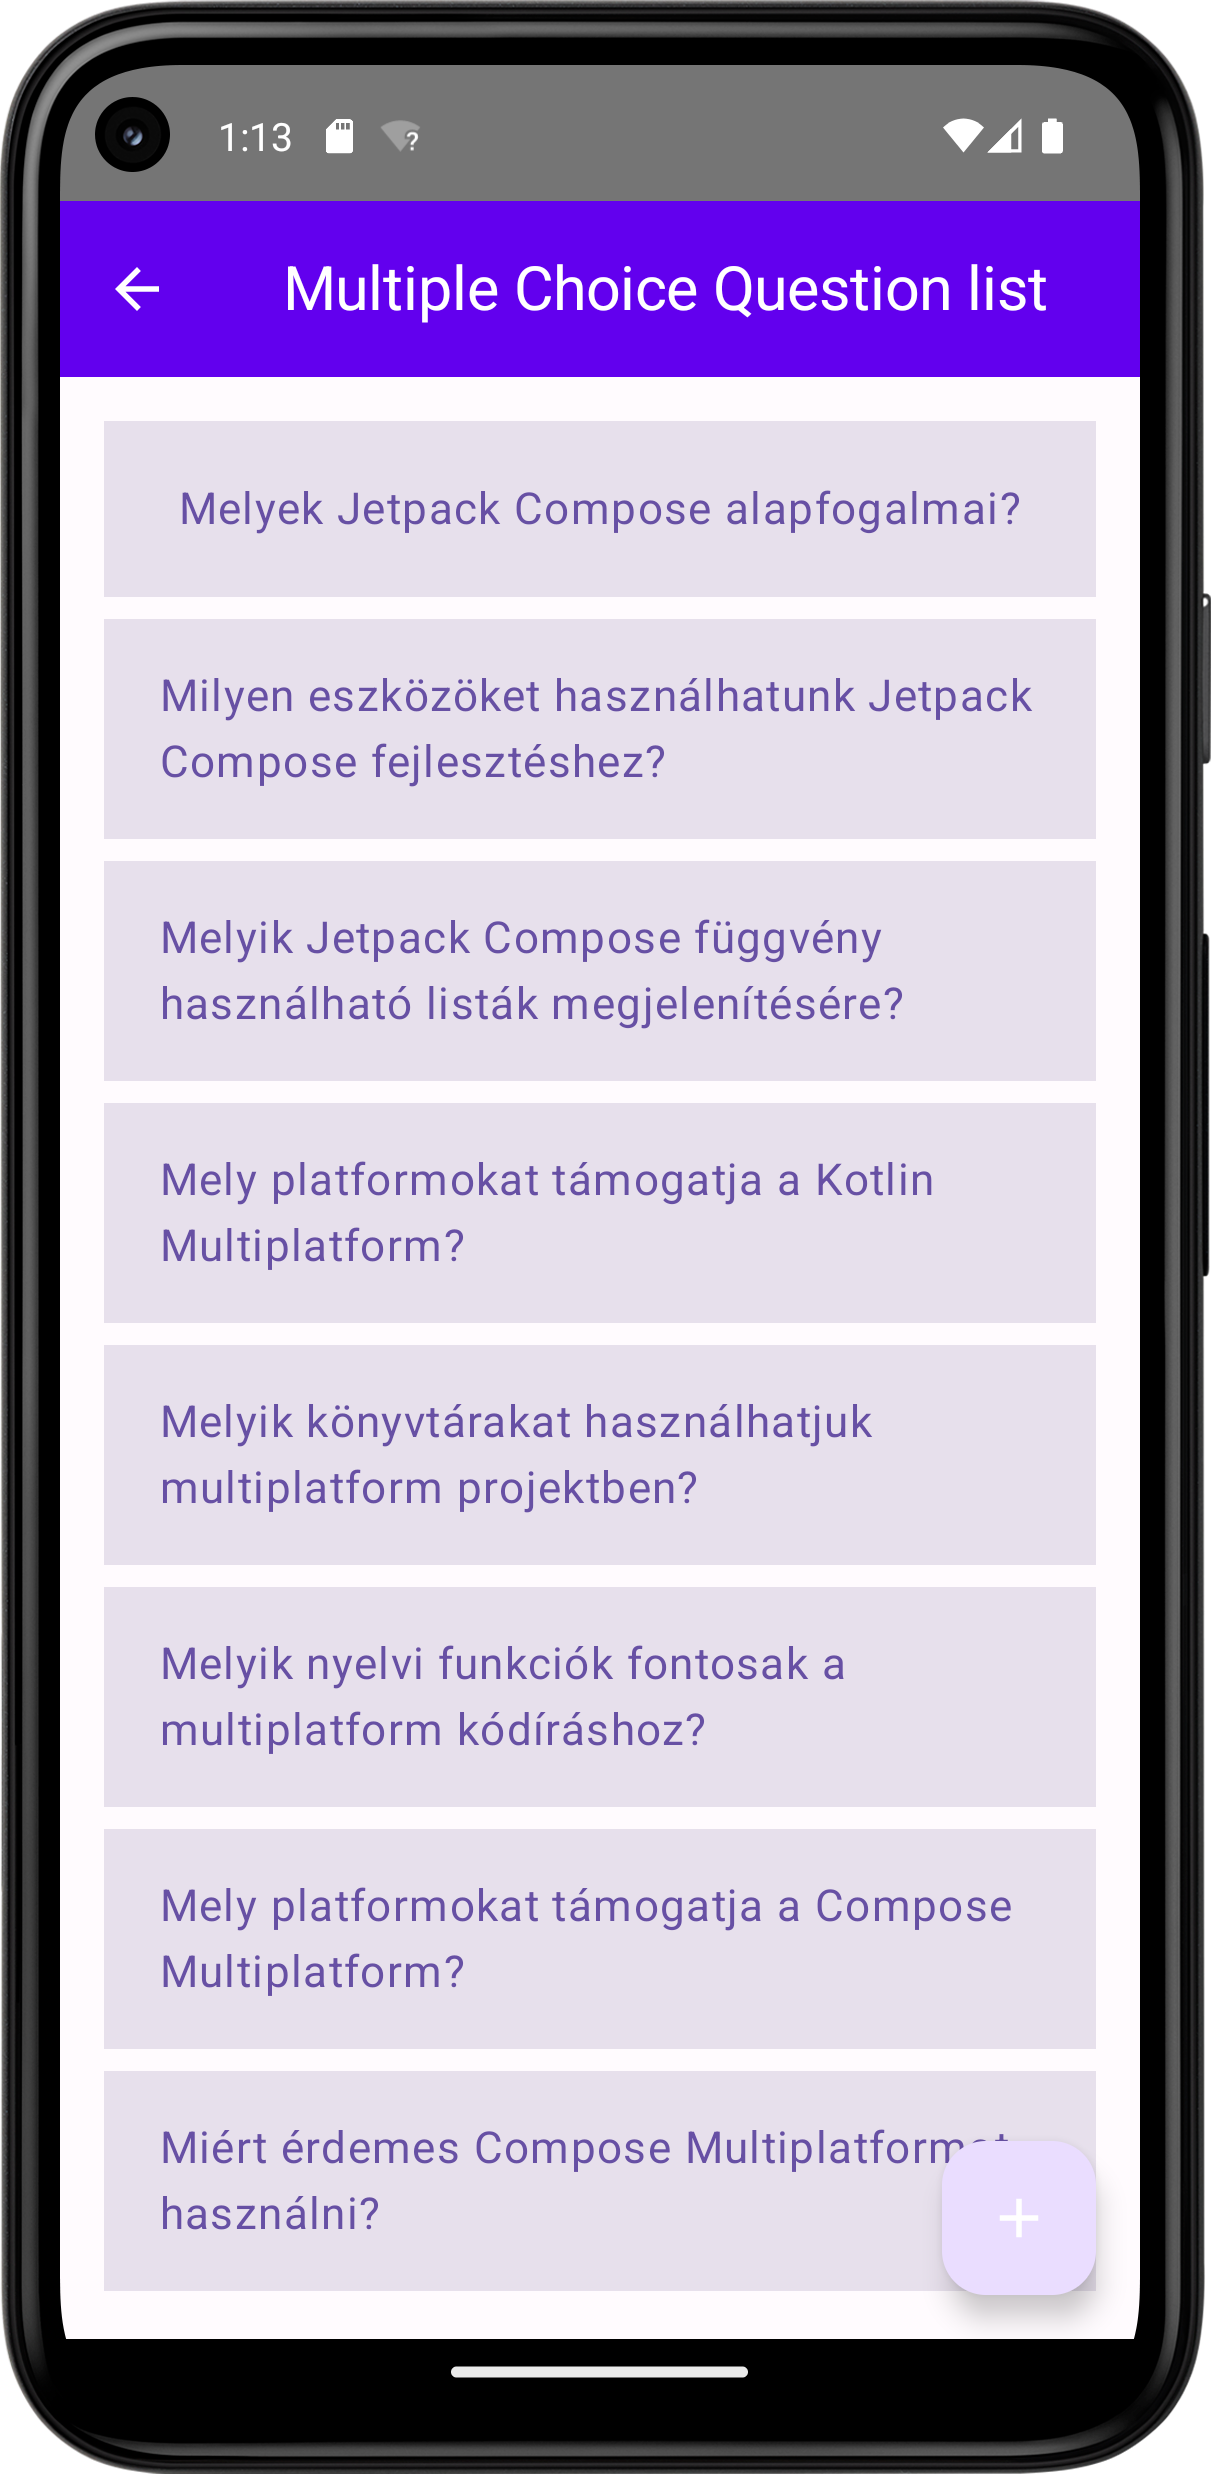
\includegraphics[width=0.3\textwidth, keepaspectratio]{figures/List_Android.png} & 
        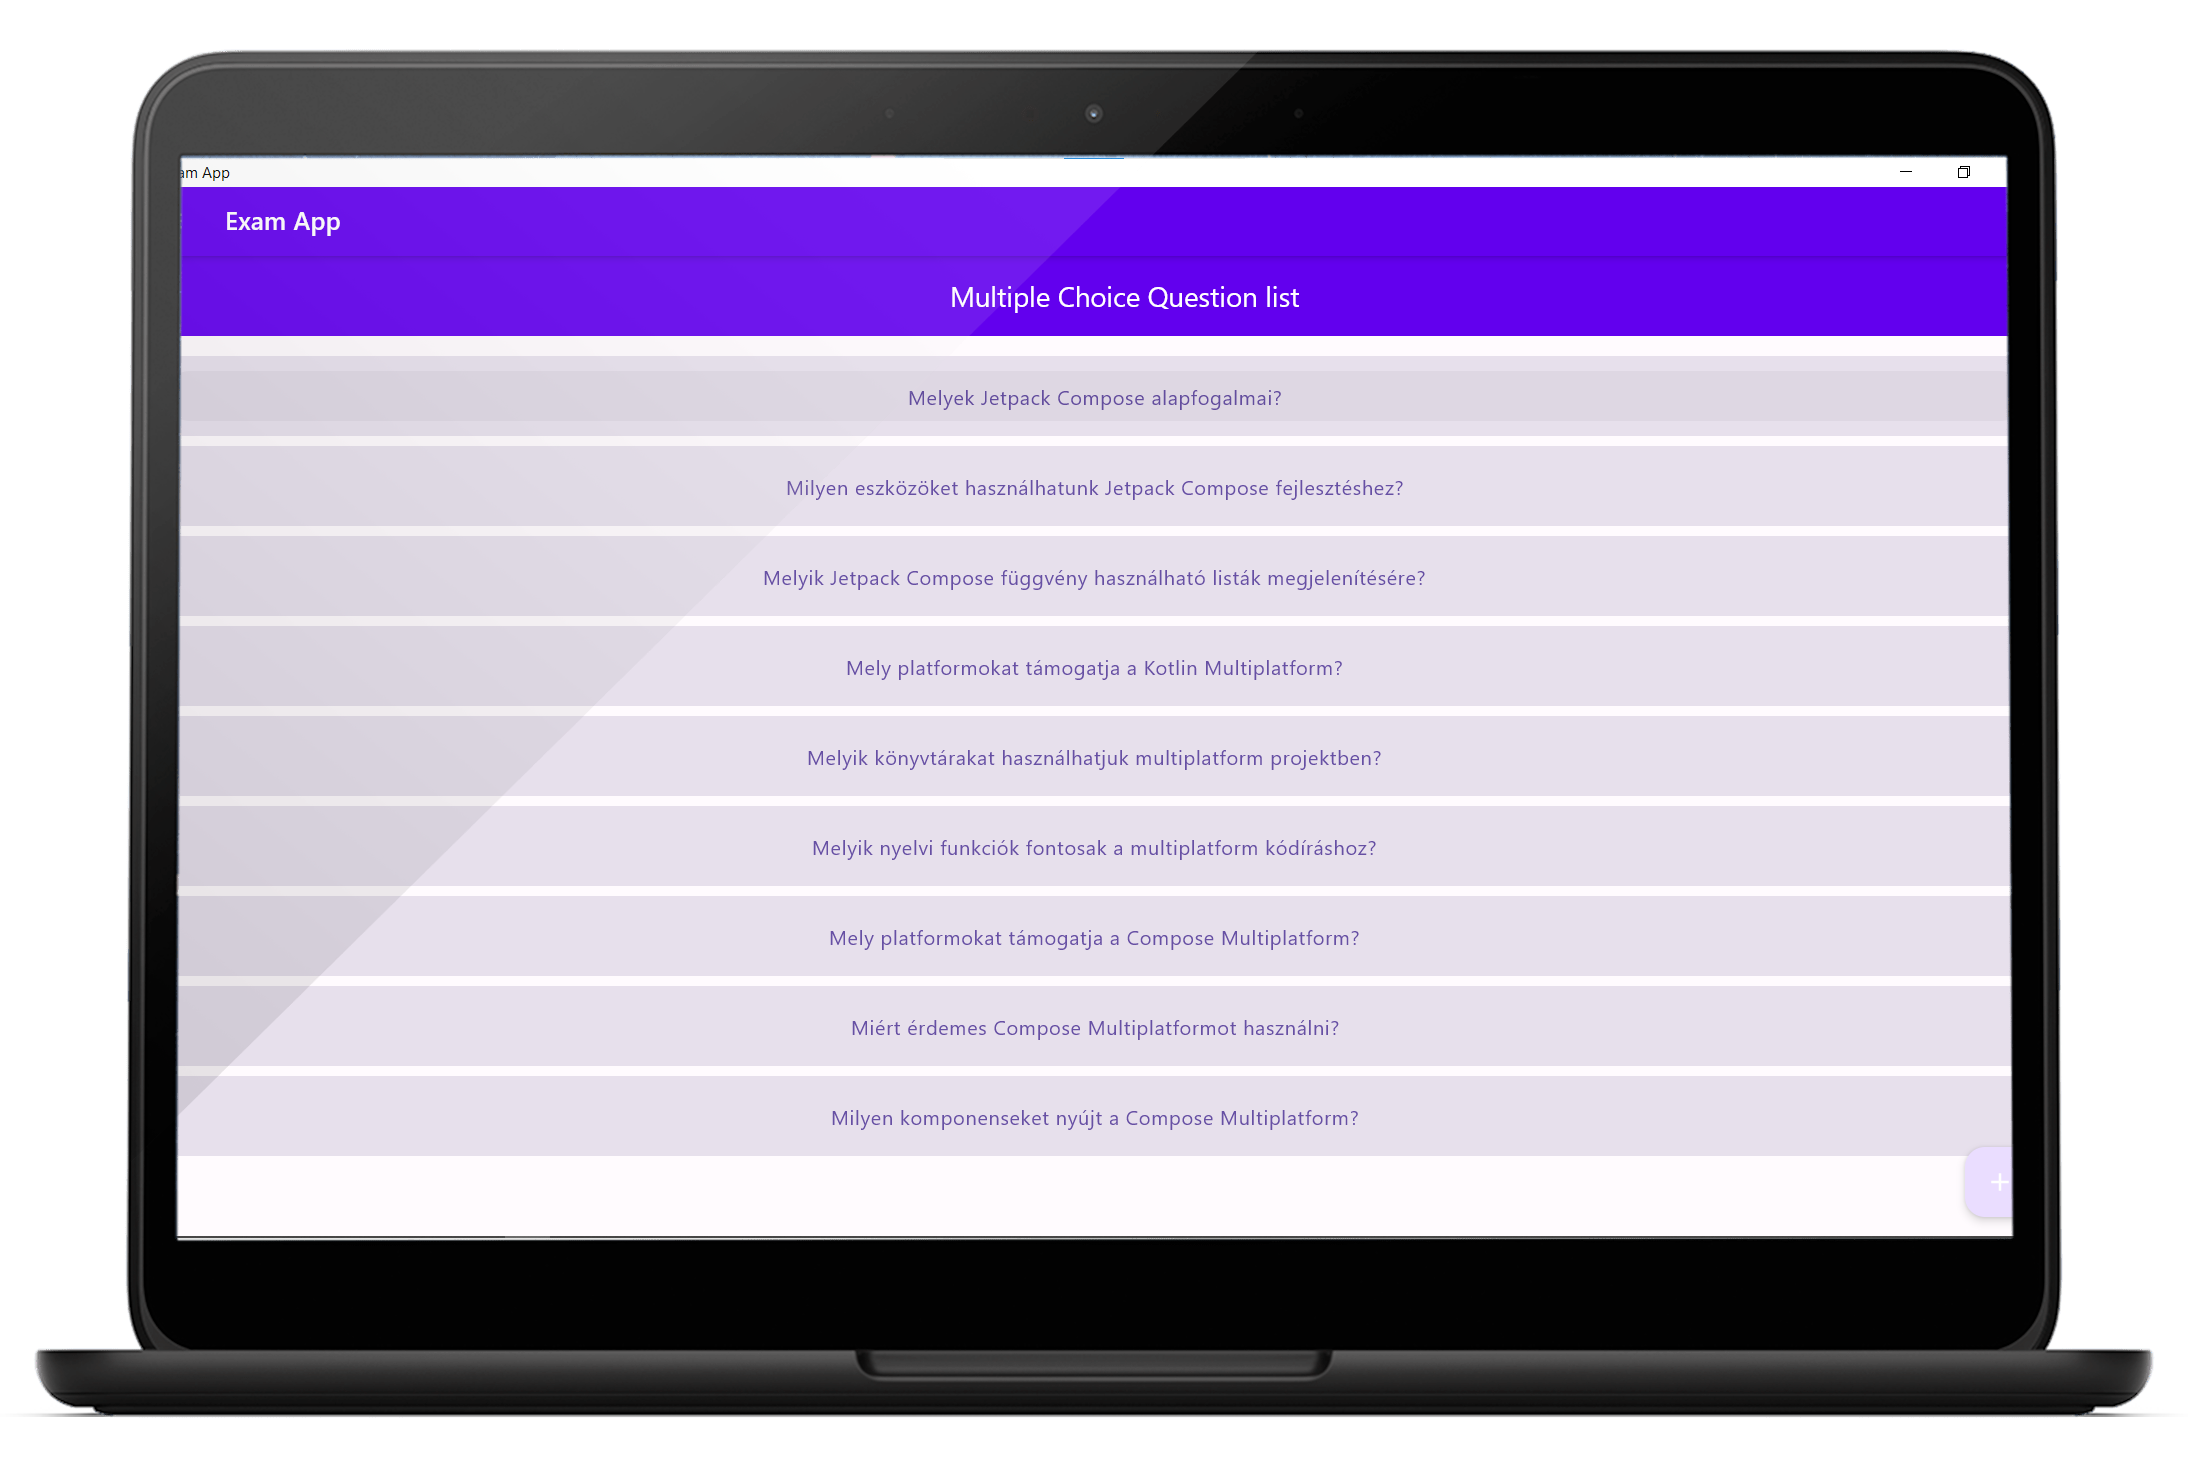
\includegraphics[width=0.6\textwidth, keepaspectratio]{figures/ListView_Desktop_framed.png}
    \end{tabular}
    \caption{A listázó képernyő Android és asztali alkalmazáson}
    \label{fig:ListScreen}
\end{figure}


\subsubsection{Részletes nézet}

A részletes oldalak általában csak az összes adatot felsorolják és mutatják meg a felhasználónak.
Ezen kívül tartalmaznak egy törlés opcióját, mivel a törlés végleges.
Továbbá innen átmehetünk a szerkesztő oldalra is.

A \refstruc{fig:DetailsScreen} egy érdekesebb megoldást mutat be.
Az oldal tetején a szokásos navigációs sávon kívül elhelyezkedik egy, a kérdések közötti keresést segítő rész.
Szűrhetünk kérdéstípusokra, ezt a csúszka segítségével tehetjük meg, ez egyúttal át is színezi őket, hogy könnyebben megkülönböztethetők legyenek.
Ezen kívül szűrhetünk témákra is.
Az utolsó dropdown menü segítségével választhatunk ki egy kérdést, amit a gombbal hozzáadhatunk a listához.

A lista része szintén LazyColumn alapú, itt a kérdések típusa alapján vannak színezve.
A kérdésekre kattintva lenyílnak, és megnézhetjük a legfontosabb adataikat, és innen is lehet törölni a kérdéseket a listából. Ezzel csak a számonkérésből törlődnek, nem a teljes adatbázisból.
Hosszan lenyomva az elemet, elhúzhatjuk felfelé és lefelé, így szabadon átrendelhetjük a kérdések sorrendjét.

\pagebreak

\begin{lstlisting}[caption={Kinyitható kérdés megvalósítása.}, label={lst:DetailsScreen}, language=Kotlin]
@Composable
fun ExpandableQuestionItem(...){
    var expandedState by remember { mutableStateOf(false) }
    val rotationState by animateFloatAsState(
        targetValue = if (expandedState) 180f else 0f, label = ""
    )
    val coroutineScope = rememberCoroutineScope()
    Card(
        modifier = Modifier.fillMaxWidth()
            .animateContentSize(
                animationSpec = tween(
                    durationMillis = 300,
                    easing = LinearOutSlowInEasing)),
        onClick = { expandedState = !expandedState}
    ) {
        Row(modifier = Modifier.background(if(question.typeOrdinal == Type.trueFalseQuestion.ordinal) PaleDogwood else Green)) {
            Column(...) {
                when (question.typeOrdinal) {
                    Type.trueFalseQuestion.ordinal -> {
                        val trueFalseQuestion = question as TrueFalseQuestionDto
                        if (expandedState) {
                            TrueFalseQuestionDetails(
                                trueFalseQuestion = trueFalseQuestion.toTrueFalseQuestionDetails(...),
                                modifier = Modifier.fillMaxWidth(),
                                colors = CardDefaults.cardColors(
                                    containerColor = PaleDogwood,
                                    contentColor = Purple40
                                )
                            )
                            RemoveButton(coroutineScope, examViewModel, question)
                        } else {
                            CollapsedQuestion(
                                question = trueFalseQuestion.question,
                                containerColor = PaleDogwood, contentColor = Purple40
                        )}}
                    Type.multipleChoiceQuestion.ordinal -> {...}
                }}
                IconButton(modifier = Modifier.weight(1f).alpha(0.2f).rotate(rotationState),
                    onClick = {expandedState = !expandedState}) {
                    Icon(
                        imageVector = Icons.Default.ArrowDropDown,
                        contentDescription = "Drop-Down Arrow"
                )}
        }}}
\end{lstlisting}

A fenti kódrészletben sok érdekes megoldás látható.
Az elején felveszünk több State-et, de ezek közül a második a legizgalmasabb. Ez a State lesz az egyik fontos eleme az animációnak.
Felhasználjuk benne az első State-et, aminek az állapota a kérdésre kattintáskor változik, és ennek az értéktől függően (nyitott vagy zárt) változtatjuk az animációhoz tartozó értéket.
A Card Composable elemen használjuk az animációt, ezt az animateContentSize segítségével tehetjük meg.
Vannak más fajta animációk is, mindegyik testreszabható, és sajátok is létrehozhatók. Ez esetben egy tween animációt használunk, ami 0.3 másodperc alatt az összecsukott állapotról egy nyitott állapotra áll át.
Attól változik meg az elem, és játszódik le az animáció, hogy rákattintunk a kérdésre.
Mivel a Card-on az animateContentSize-t használtuk, ezért amikor az expandedState megváltozik, akkor a CollapsedQuestion helyett a TrueFalseQuestionDetails-nek kell megjelenni, ez méretváltozással jár, ezt követi le az animáció, így nem hirtelen ugrik egyet a képernyő, hanem lekövethető módon változik meg.
A rotationState pedig az ArrowDropDown elem animálásában játszik szerepet, így az ikont el tudjuk forgatni 180 fokkal, ehhez a Modifierhez tartozó rotate() extension function-t tudjuk használni.

\begin{figure}[!ht]
    \centering
    \begin{tabular}{cc}
        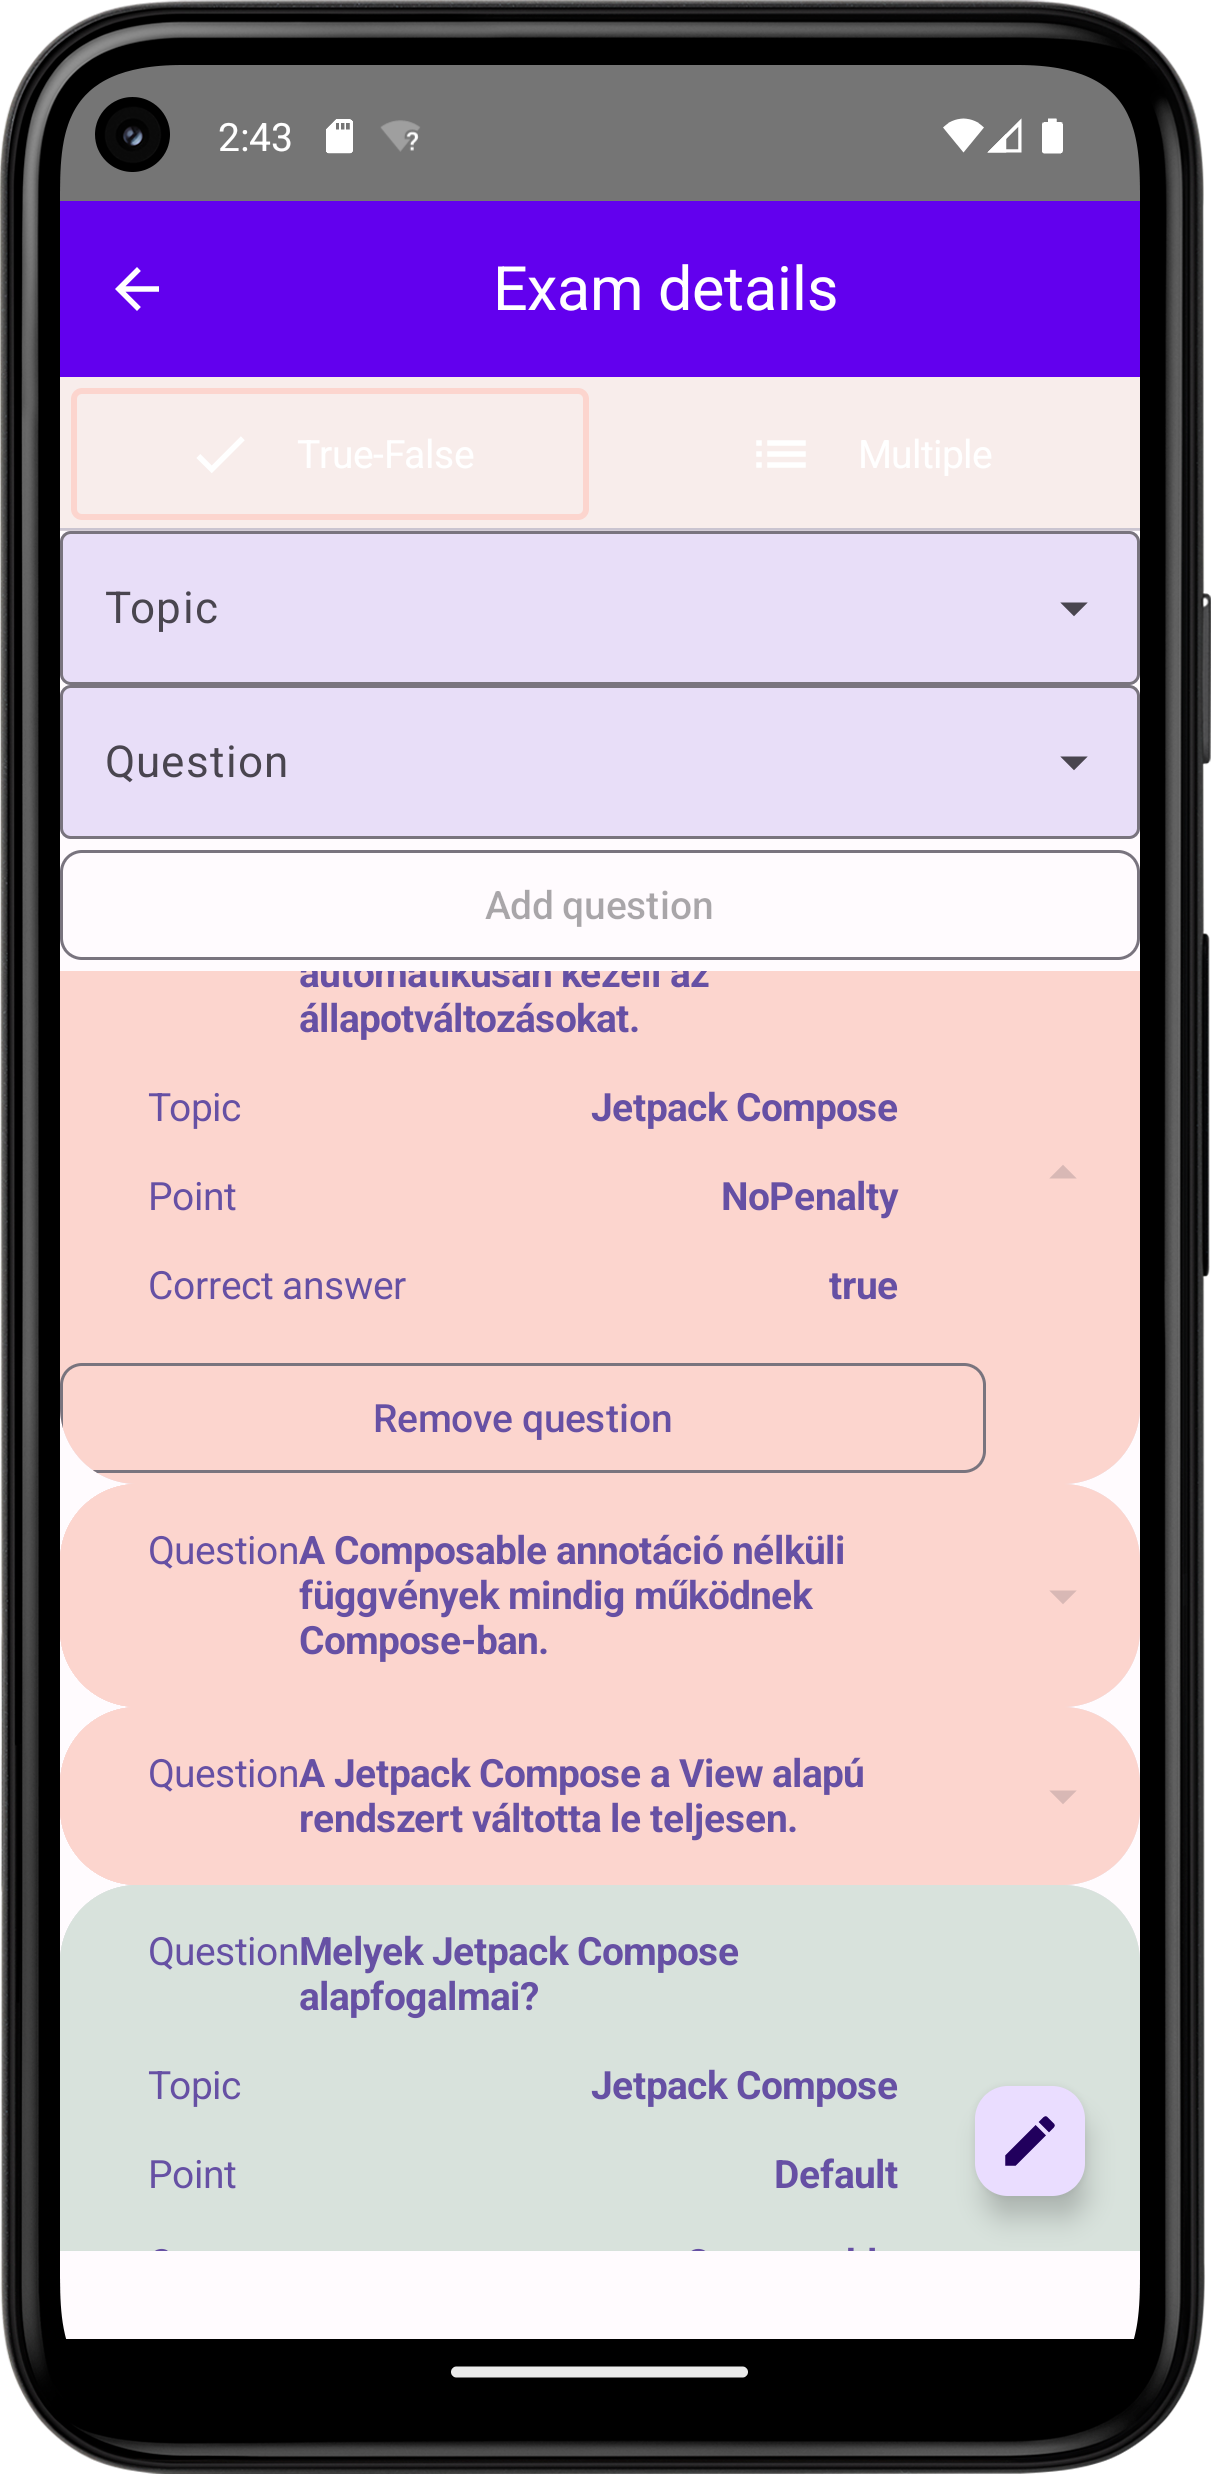
\includegraphics[width=0.3\textwidth, keepaspectratio]{figures/Details_Android.png} & 
        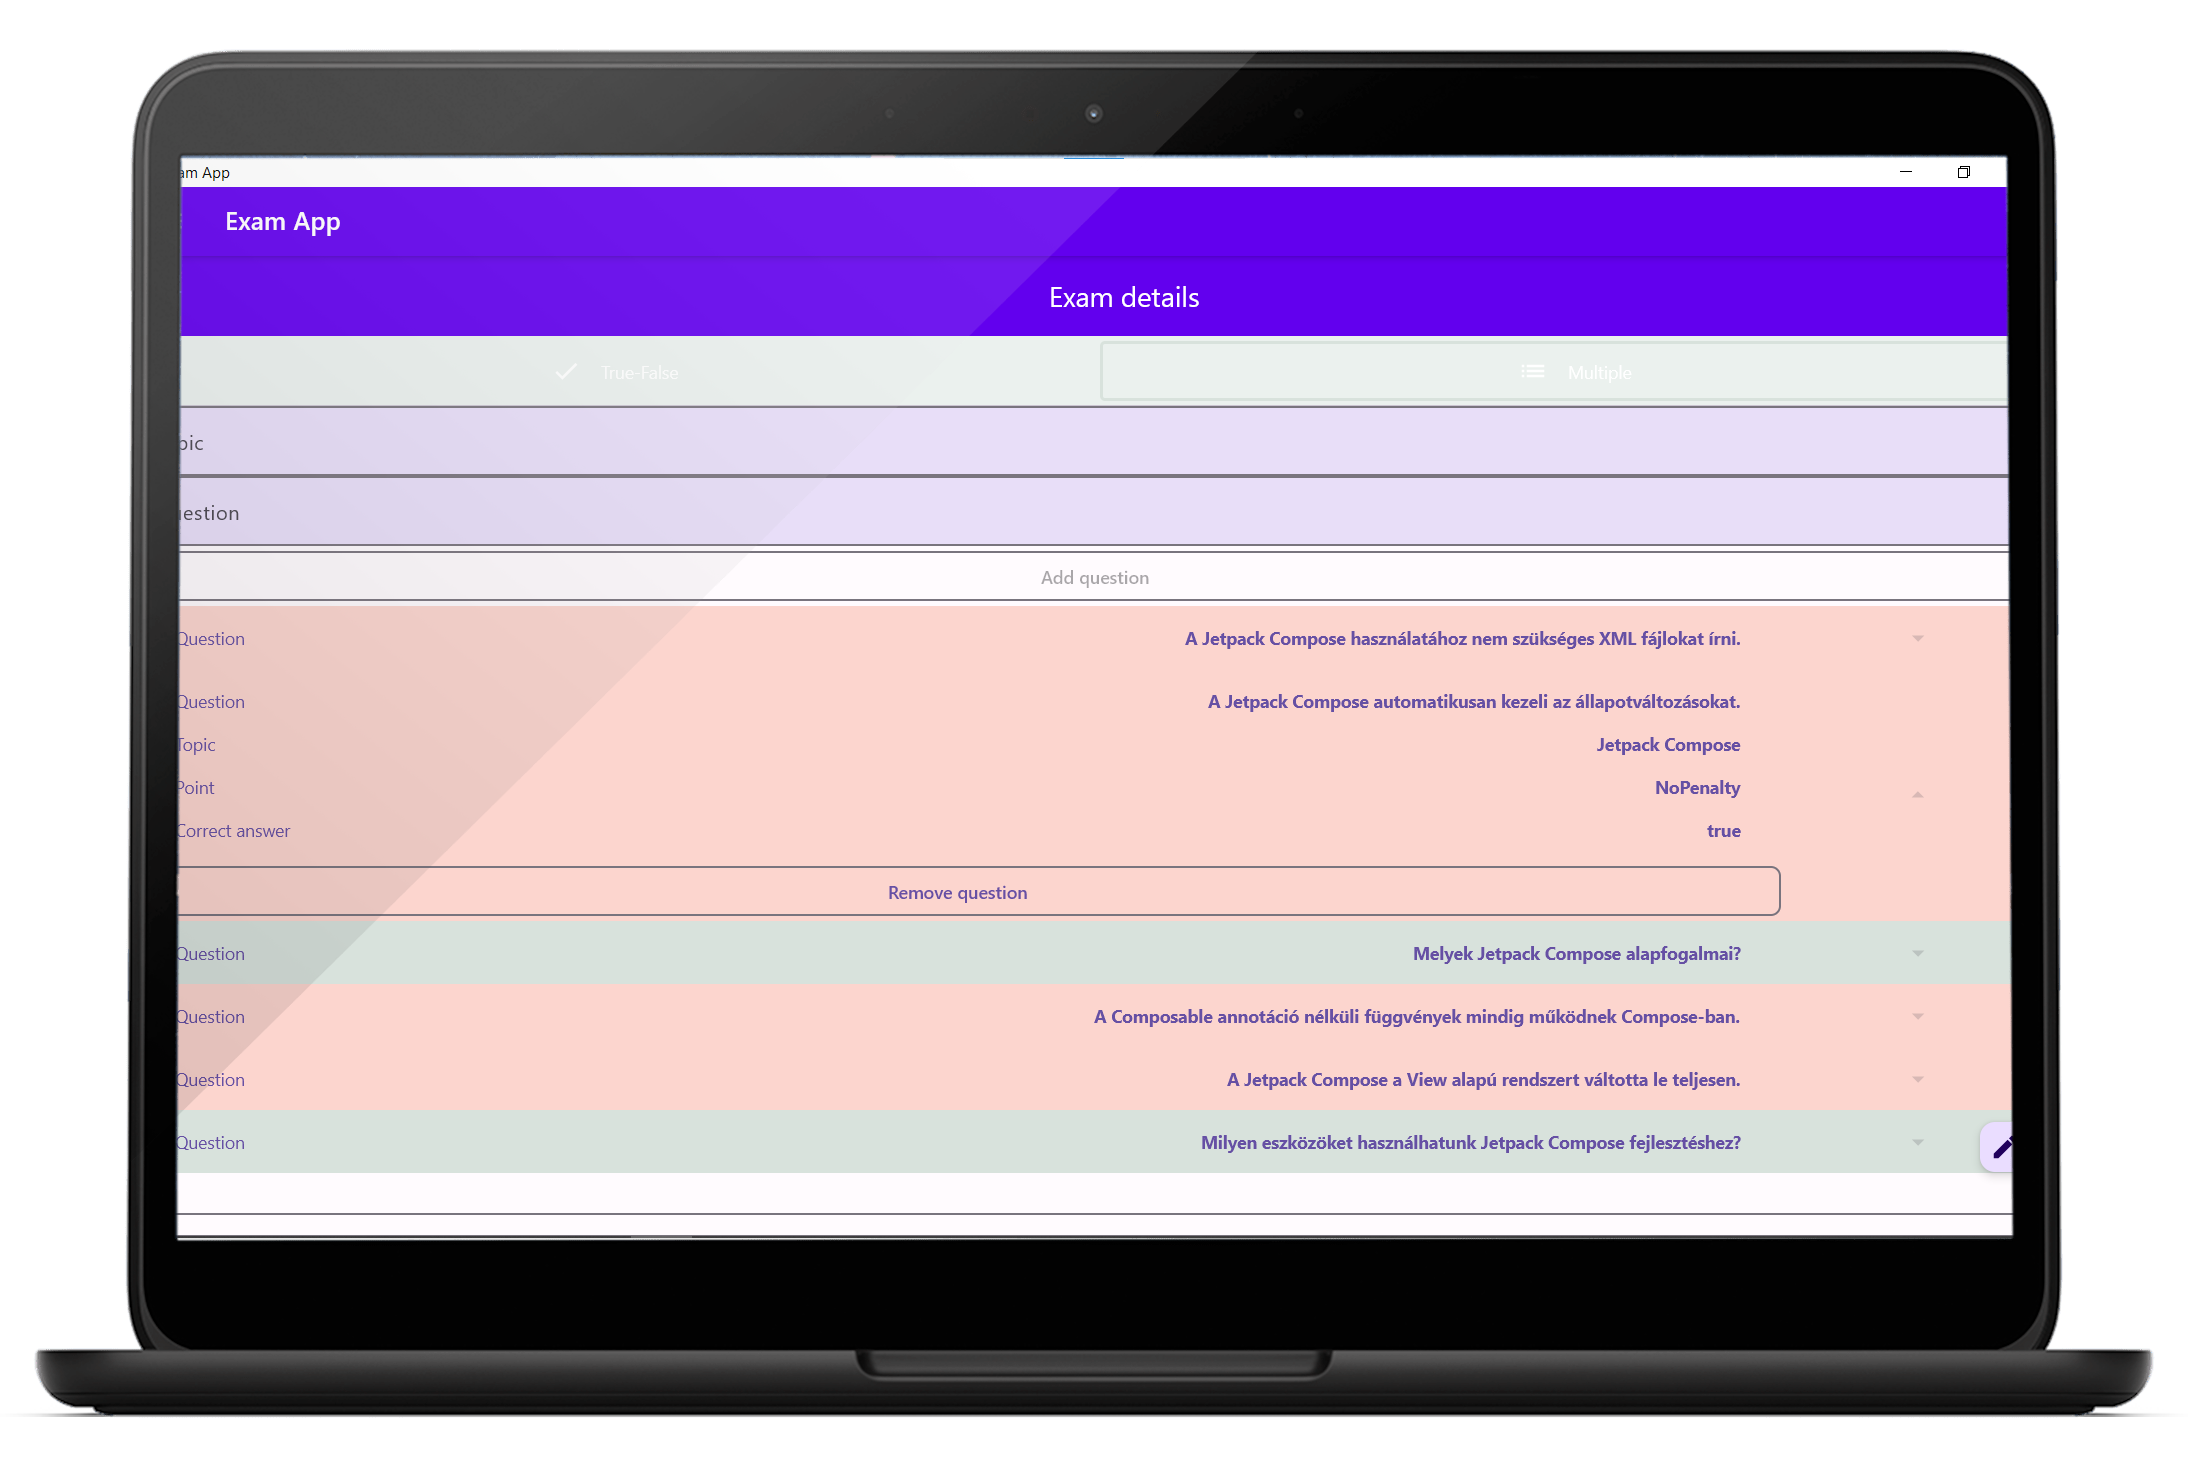
\includegraphics[width=0.6\textwidth, keepaspectratio]{figures/Details_Desktop_framed.png}
    \end{tabular}
    \caption{Egy érdekesebb részletes képernyő, a vizsgák összeállításához tartozik.}
    \label{fig:DetailsScreen}
\end{figure}


\subsubsection{Szerekesztő nézet}

\begin{figure}[!ht]
    \centering
    \begin{tabular}{cc}
        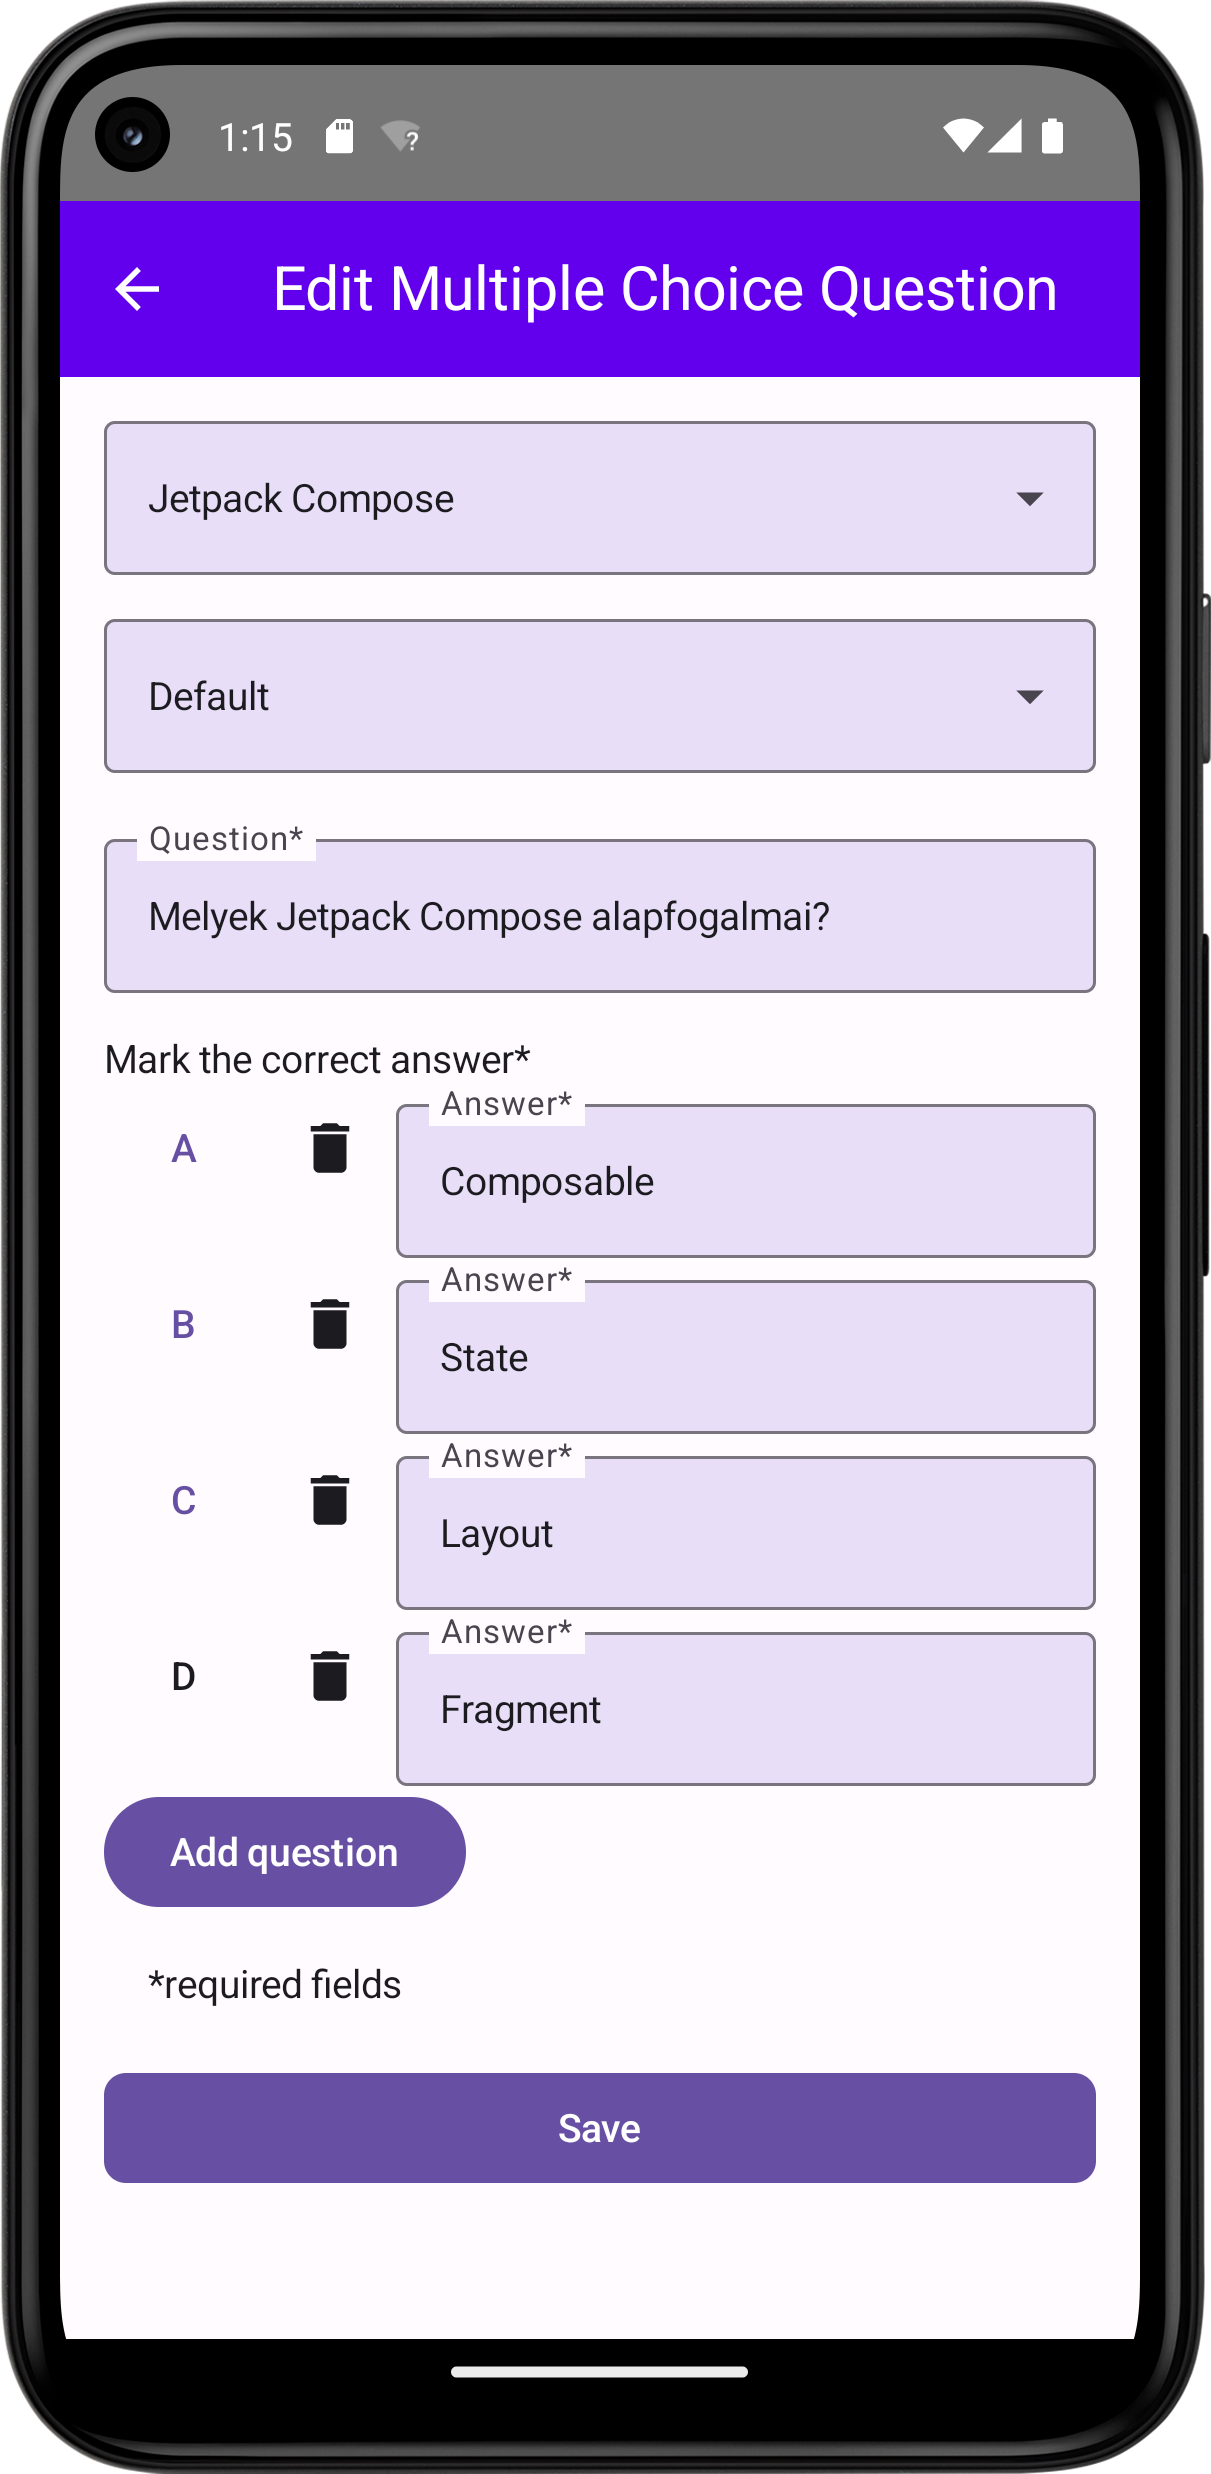
\includegraphics[width=0.3\textwidth, keepaspectratio]{figures/Edit_Android.png} & 
        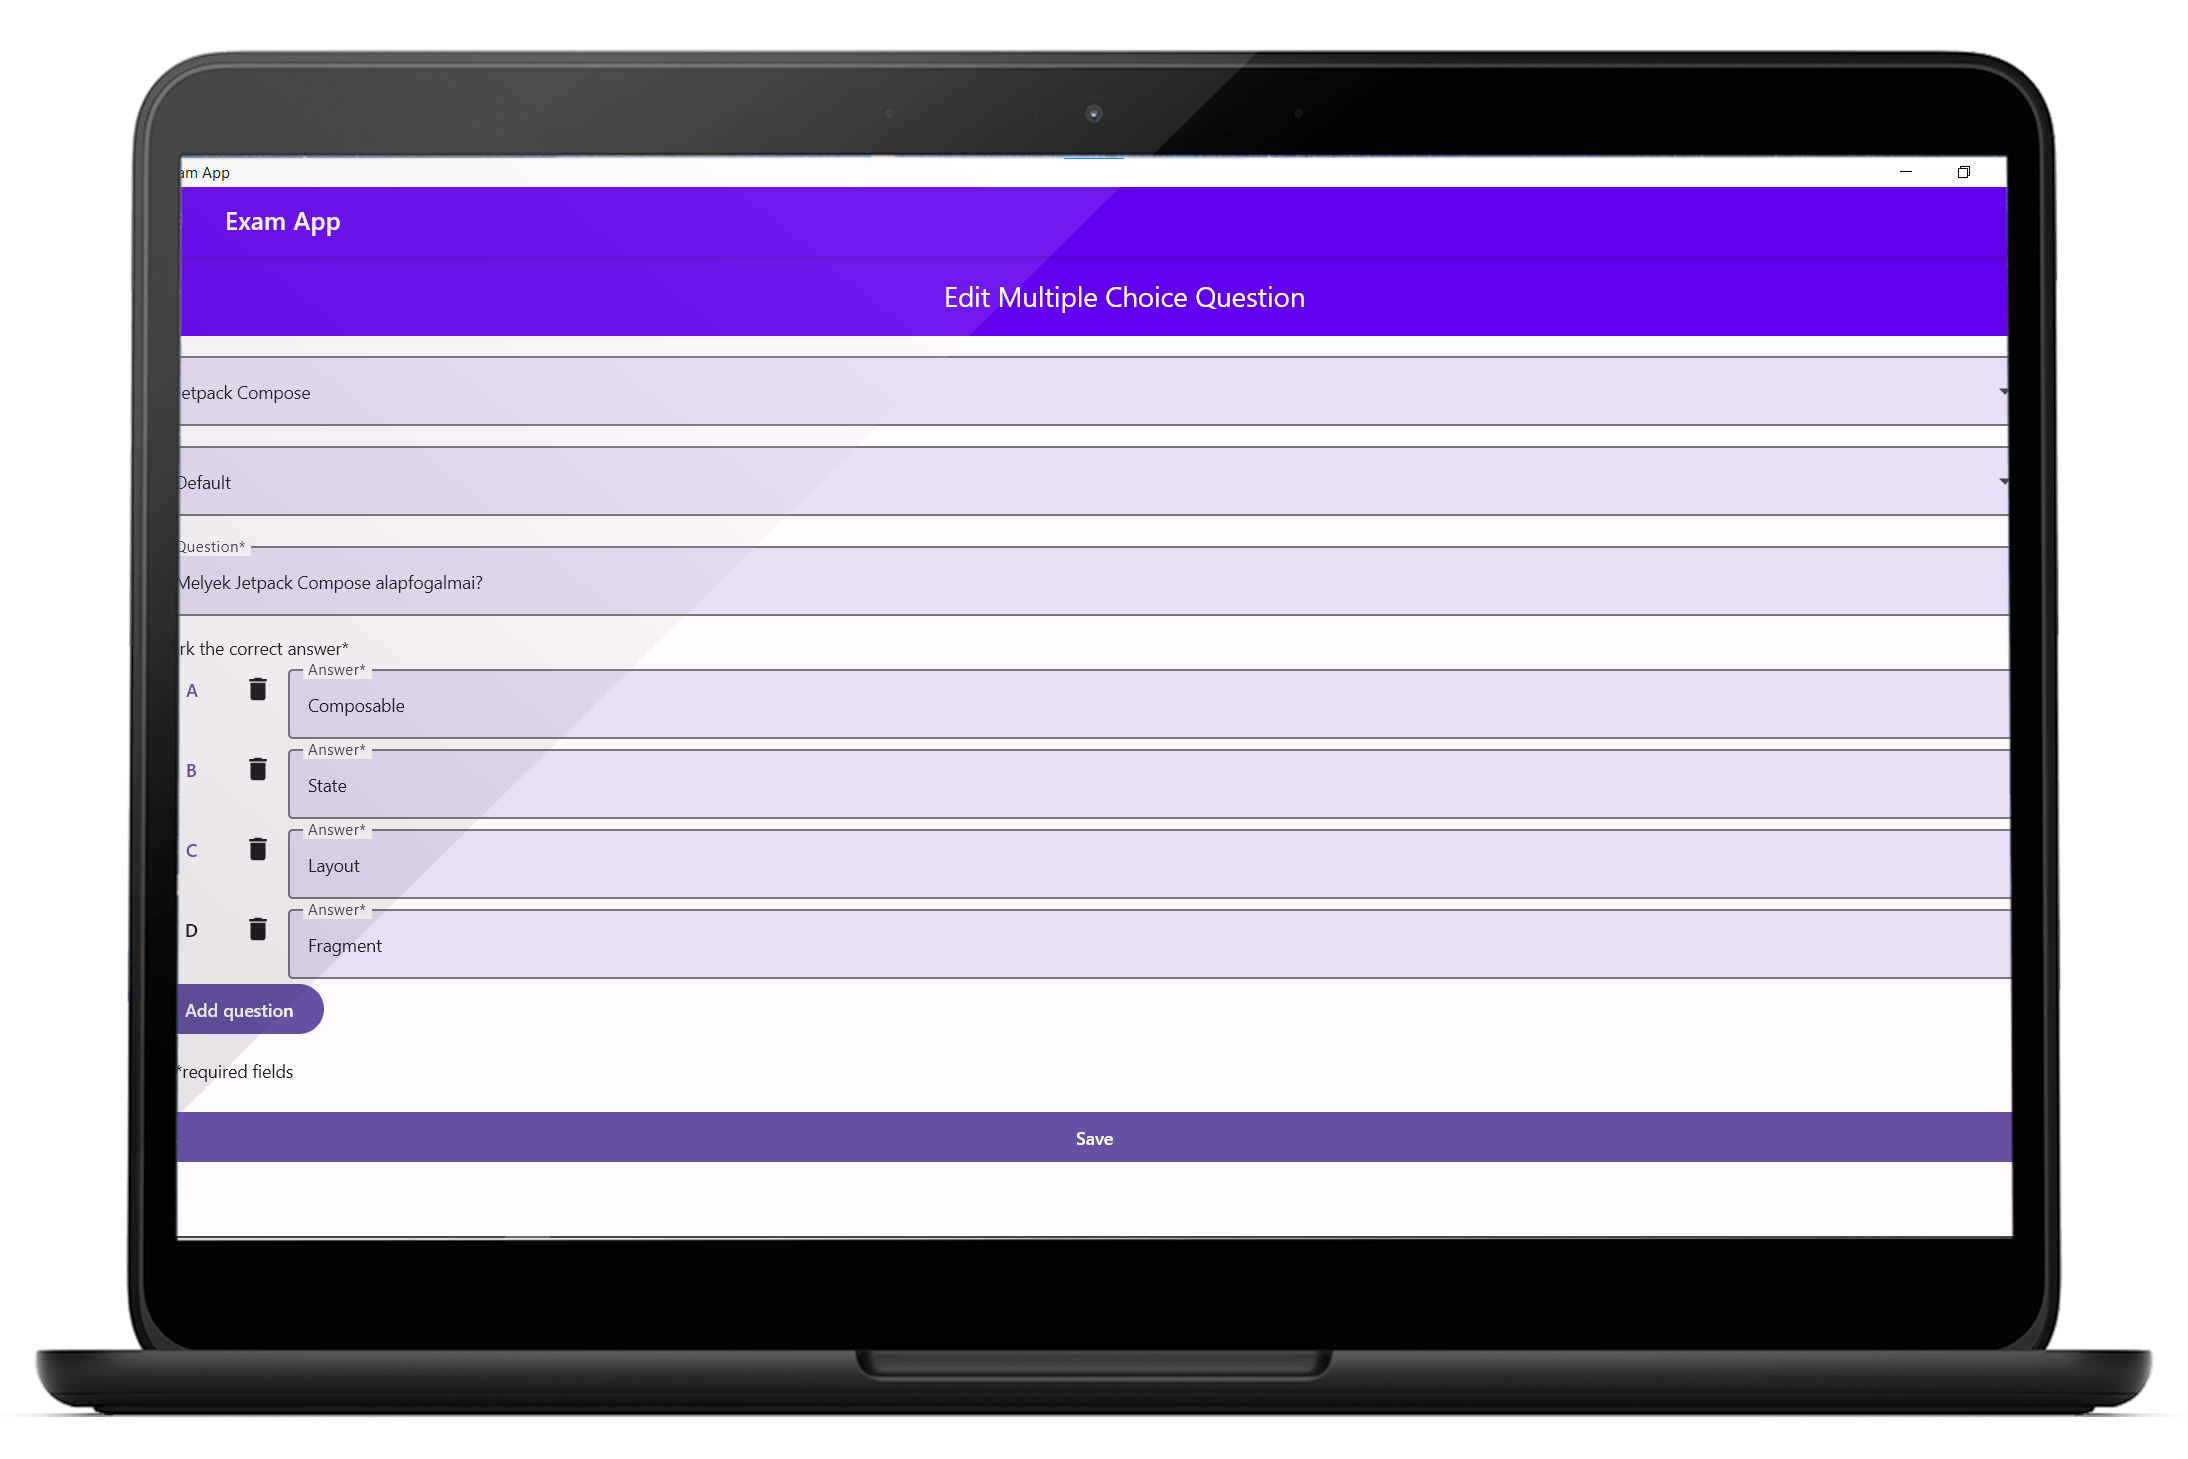
\includegraphics[width=0.6\textwidth, keepaspectratio]{figures/Edit_Desktop_framed.png}
    \end{tabular}
    \caption{Egy érdekesebb szerkesztő képernyő, a feleltválasztós kérdések létrehozásához.}
    \label{fig:EditScreen}
\end{figure}

A szerkesztő nézetben lehet módosítani minden adatot (kivéve a feladatsorhoz tartozó kérdéseket, amit az előző alfejezetben mutattam be).
Itt sokféle elem megtalálható: szöveges beviteli mezők, dropdown menü, a pontok esetében pedig numerikus beviteli mezők.

A feleletválasztós kérdéseknél (\refstruc{fig:EditScreen}) van egy speciális elem, ami a kérdések megadásához készült.
Tartalmaz egy TextButton-t, ami a válasz sorszáma, egy ImageButton-t a válasz törléséhez és egy szöveges beviteli mezőt a válasz megadásához.
Tetszőleges opció megadható, itt viszont egy egyszerű Column mellett döntöttem, és egy for ciklus segítségével rajzolom ki az elemeket.


\begin{lstlisting}[caption={Szerkesztő nézet kódja.}, label={lst:EditScreen}, language=Kotlin]
@Composable
fun ExamInputForm(
    enabled: Boolean = true,
    entryViewModel: ExamEntryViewModel = viewModel { ExamEntryViewModel() },    
    topicListViewModel: TopicListViewModel = viewModel { TopicListViewModel() },
    ) {
    val coroutineScope = rememberCoroutineScope()
    Column(...) {
        OutlinedTextField(
            value = examDetails.name,
            onValueChange = { onValueChange(examDetails.copy(name = it)) },
            enabled = enabled,
            ...
        )
        DropDownList(
            name = stringResource(Res.string.exam),
            items = topicListViewModel.topicListUiState.topicList.map{it.topic}.filterNot{ it == examDetails.topicName },
            onChoose = {topic ->
                coroutineScope.launch{
                    onValueChange(examDetails.copy(topicId = entryViewModel.getTopicIdByTopic(topic)))
                }
            },
            default = examDetails.topicName,
            modifier = Modifier.fillMaxWidth(),
        )
        if (enabled) {
            Text(
                text = stringResource(Res.string.required_fields),
                modifier = Modifier.padding(start = 16.dp)
            )
        }
    }
}
\end{lstlisting}

A fenti kódrészletben megfigyelhetjük a ViewModelek átadását a Composable függvénynek.
Esetenként többre is szükség lehet, itt például az examEntry és a topicList ViewModelekre is szükség van, mivel a dropdown listában a témakört ki kell választani a feladatsorhoz.
A dropdown menü kódjában kihasználtam a Kotlin funkcionális programozást segítő elemeit, ezzel kigyűjtöttem a témakörök listájából azokat, amelyek nem egyeznek meg a jelenleg kiválasztottal.
A hosszabb ideig tartó műveleteket egy coroutineScope-ban valósítottam meg egy másik lambda függvényben, így a UI nem blokkolódik le közben.
A mentés gomb le van tiltva, ha hiányzik egy kötelező mező, vagy ha ez egyedi mezőkben ütközés van, a felhasználó kap egy értesítést, és a gomb is letiltódik, amíg nem változtat az értéken.

\pagebreak

\subsubsection{Új elem létrehozása}

Ez a nézet lényegében megegyezik a szerkesztő nézettel.
Egy jó szoftver arról ismerhető meg, hogy a lehető legtöbb helyen újra felhasználja a már meglévő kódot anélkül, hogy annak a működését lényegesen meg kellene változtatnia.
Ebben az esetben már a tervezés során megszületett a döntés. Egész pontosan van egy body része az új elem felvételének, ami vár paraméterként egy UiState-et, amiben az adott elem adatai kerülnek.
Az alapértelmezett értékek úgy vannak megválasztva, hogy üres hatást keltsenek, de ha már léteznek, akkor a szerkesztő nézetet kapjuk, az új létrehozása helyett.
Ehhez szükség van külön ViewModel-re és kevés Composable függvény megírására is, de ez jelentősen kevesebb, mint az egész kód újraírása. Ezzel a kód karbantarthatósága is növekszik.

\begin{figure}[!ht]
    \centering
    \begin{tabular}{cc}
        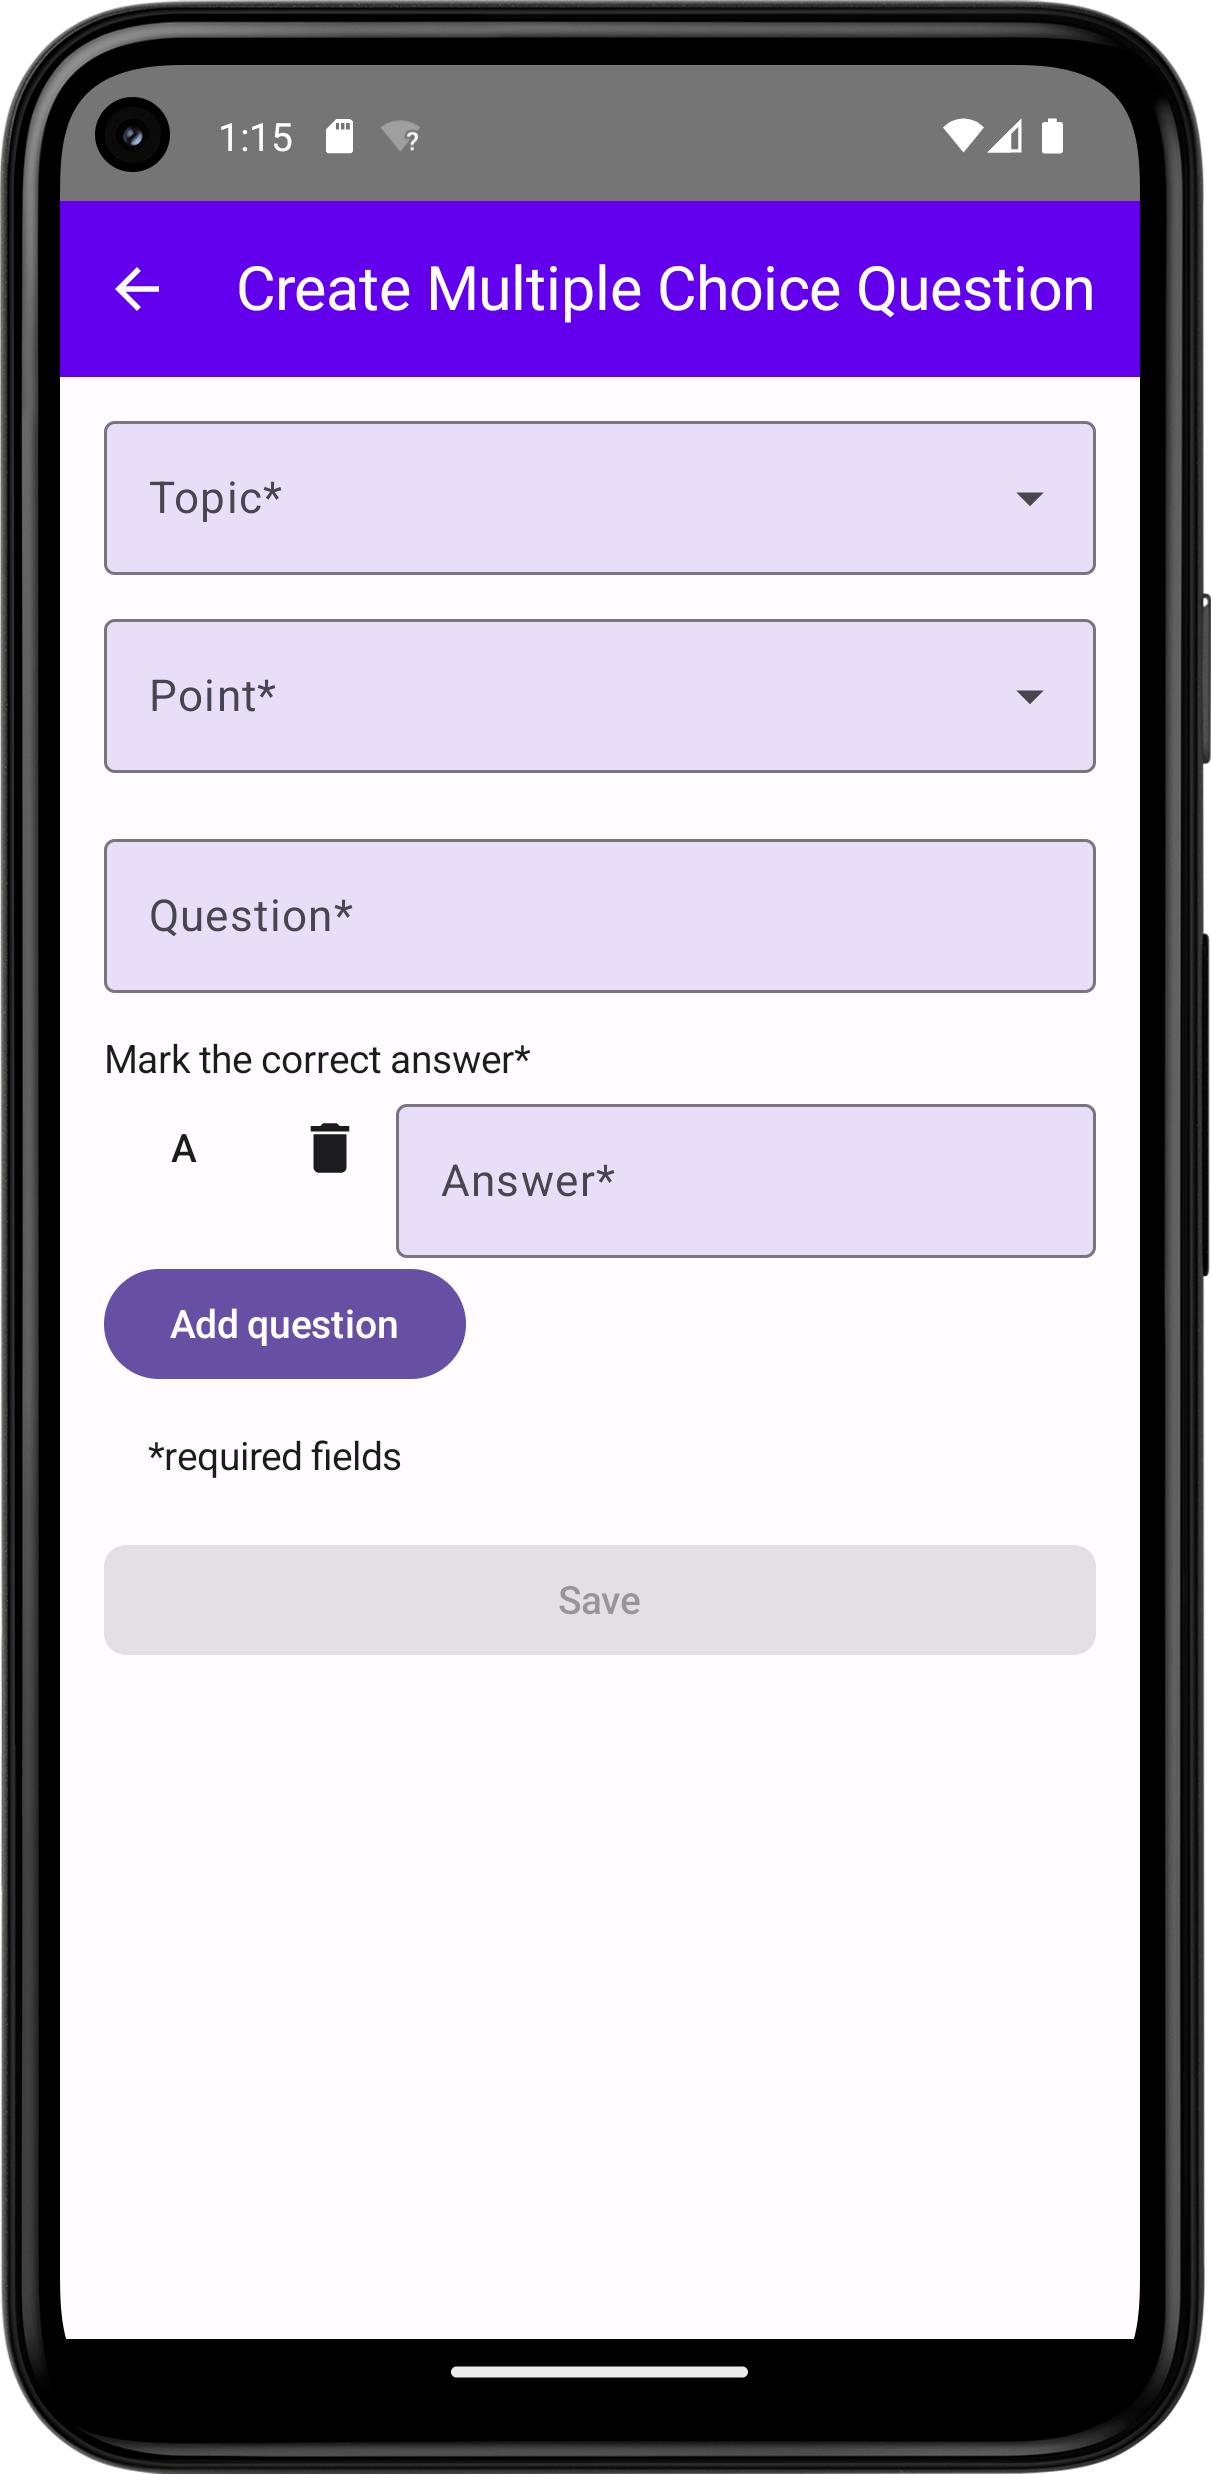
\includegraphics[width=0.3\textwidth, keepaspectratio]{figures/New_Android.png} & 
        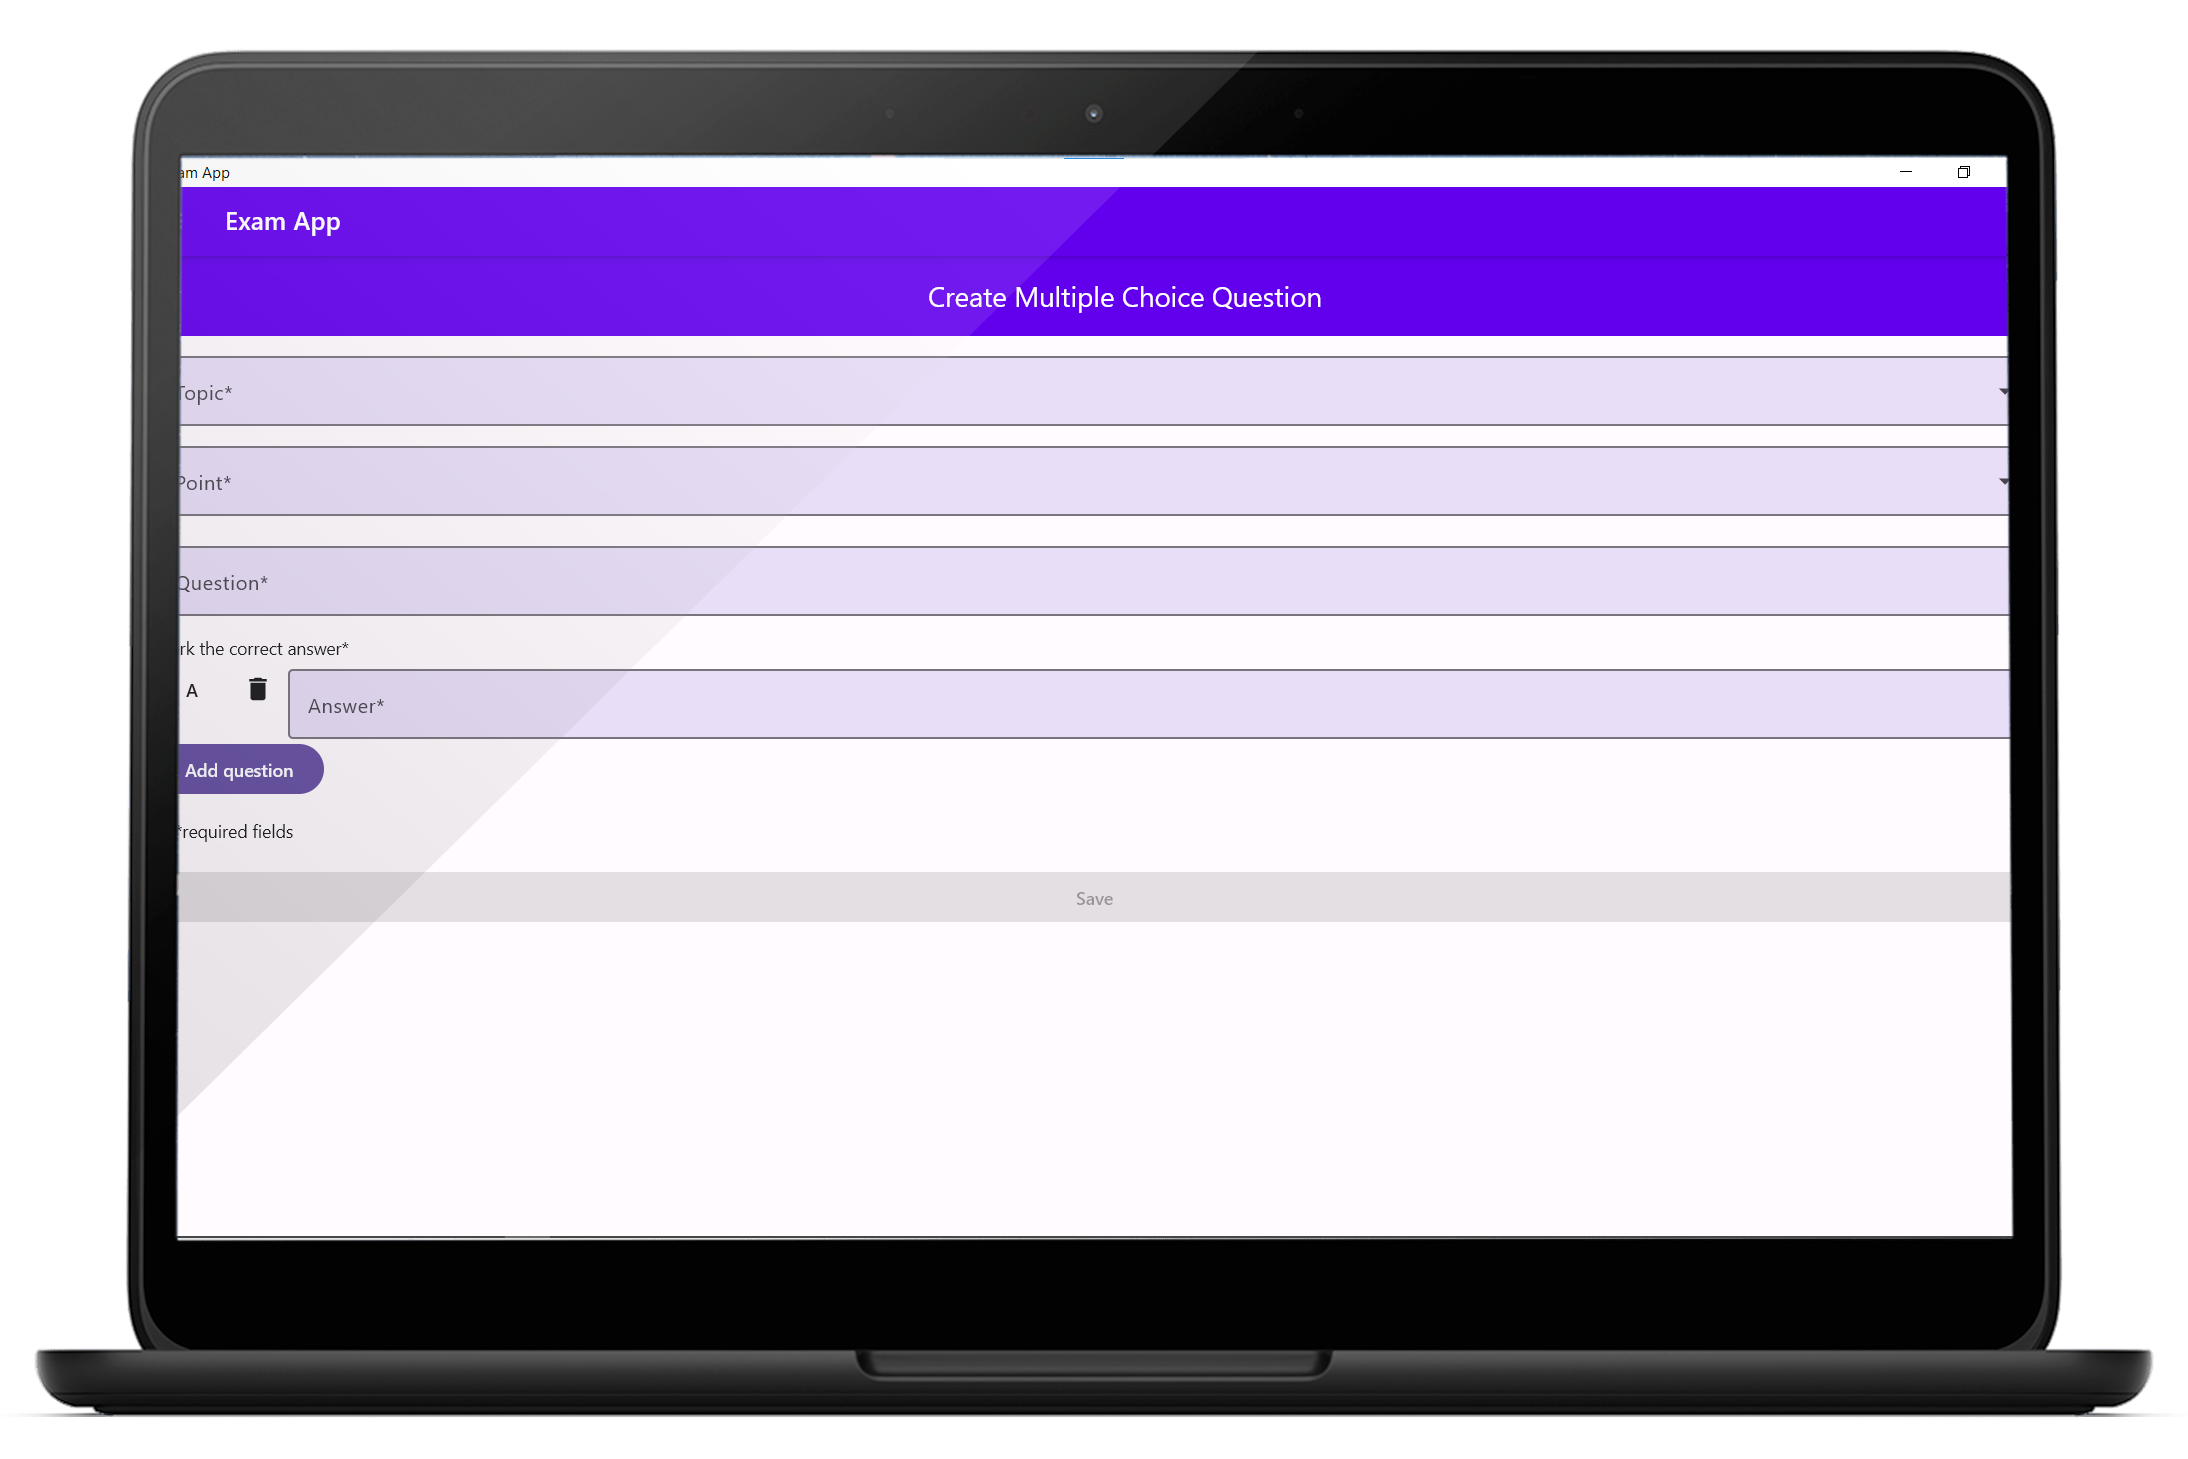
\includegraphics[width=0.6\textwidth, keepaspectratio]{figures/New_Desktop_framed.png}
    \end{tabular}
    \caption{Új feleletválasztós kérdés létrehozása.}
    \label{fig:NewScreen}
\end{figure}


\subsubsection{Ellenőrző képernyő}

Az ellenőrző képernyőn a kérdések vannak felsorolva, a szokásos színkódolással.
Olvasható a teljes szöveg és a válaszok is a feleletválasztós kérdéseknél.
A válasz formátuma látható a kitöltés előtt, így a felhasználó tudja, hogy milyen formátumban van elvárva a válasz.
A fenti Scan Exam gomb Android-eszközön megnyit egy kameranézetet, ami segítségével pár gyors mozdulattal be tudjuk olvasni a válaszokat, így nem kell kézzel begépelni azt.
Ha valamit nem vagy rosszul detektált, akkor természetesen az oldalon ezek javíthatók.
A lap alján található egy gomb, ami segítségével ki lehet értékelni a válaszokat, ez a backend oldalon történik meg, majd az eredményt visszaküldi, és a felhasználó megtekintheti az elért pontszámot és a százalékos értéket.

\begin{figure}[!ht]
    \centering
    \begin{tabular}{cc}
        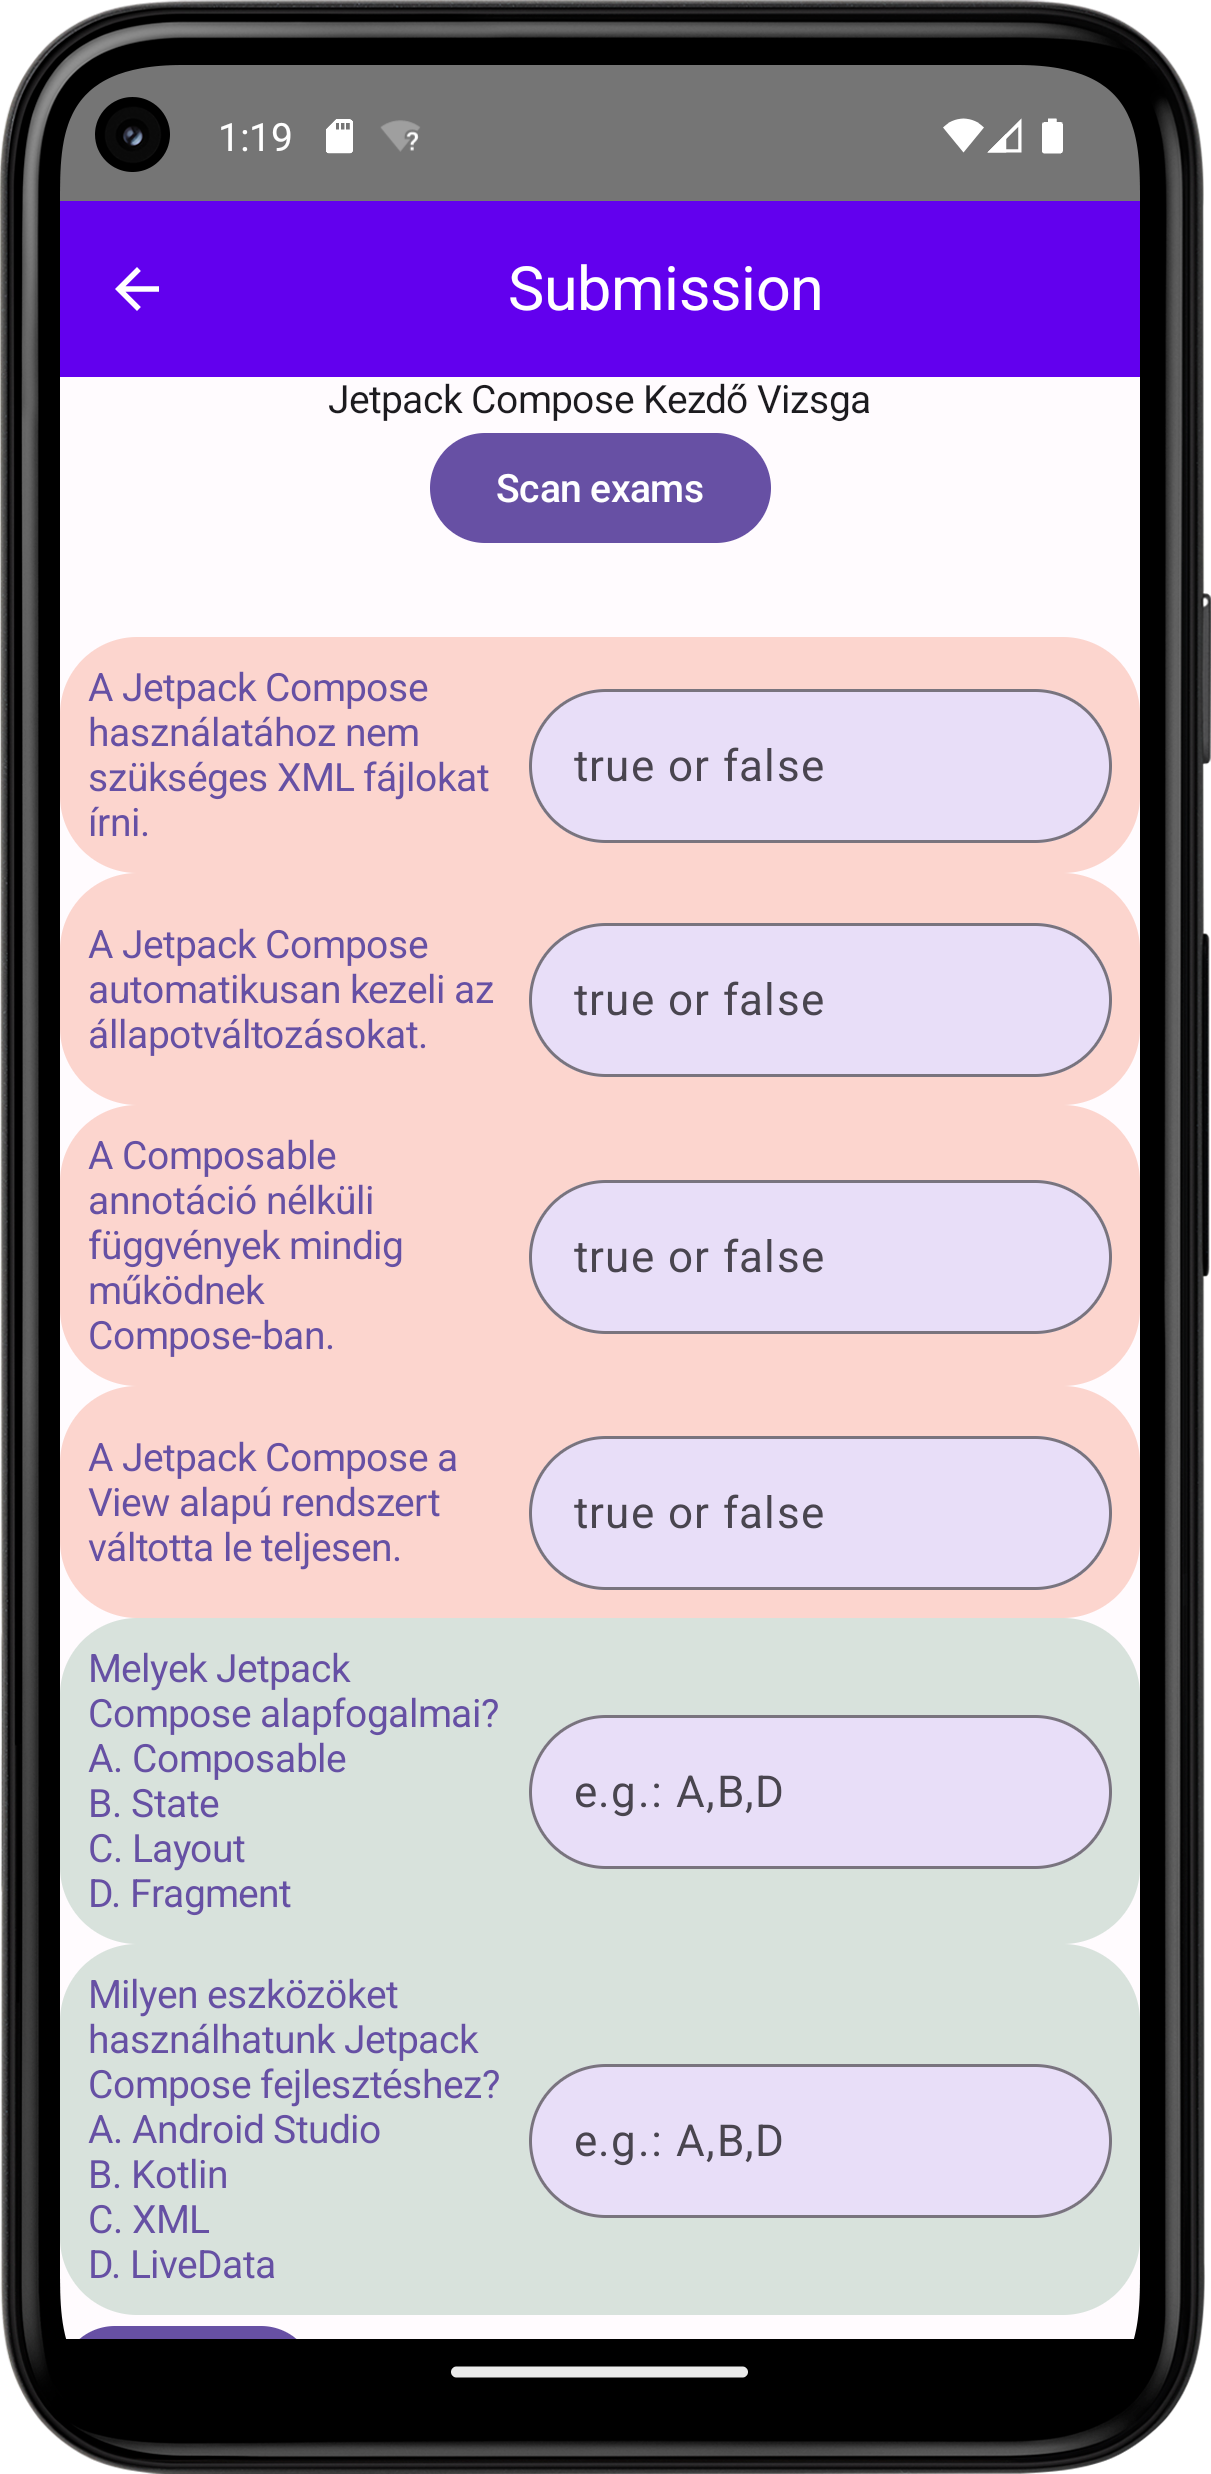
\includegraphics[width=0.3\textwidth, keepaspectratio]{figures/Submission_Android.png} & 
        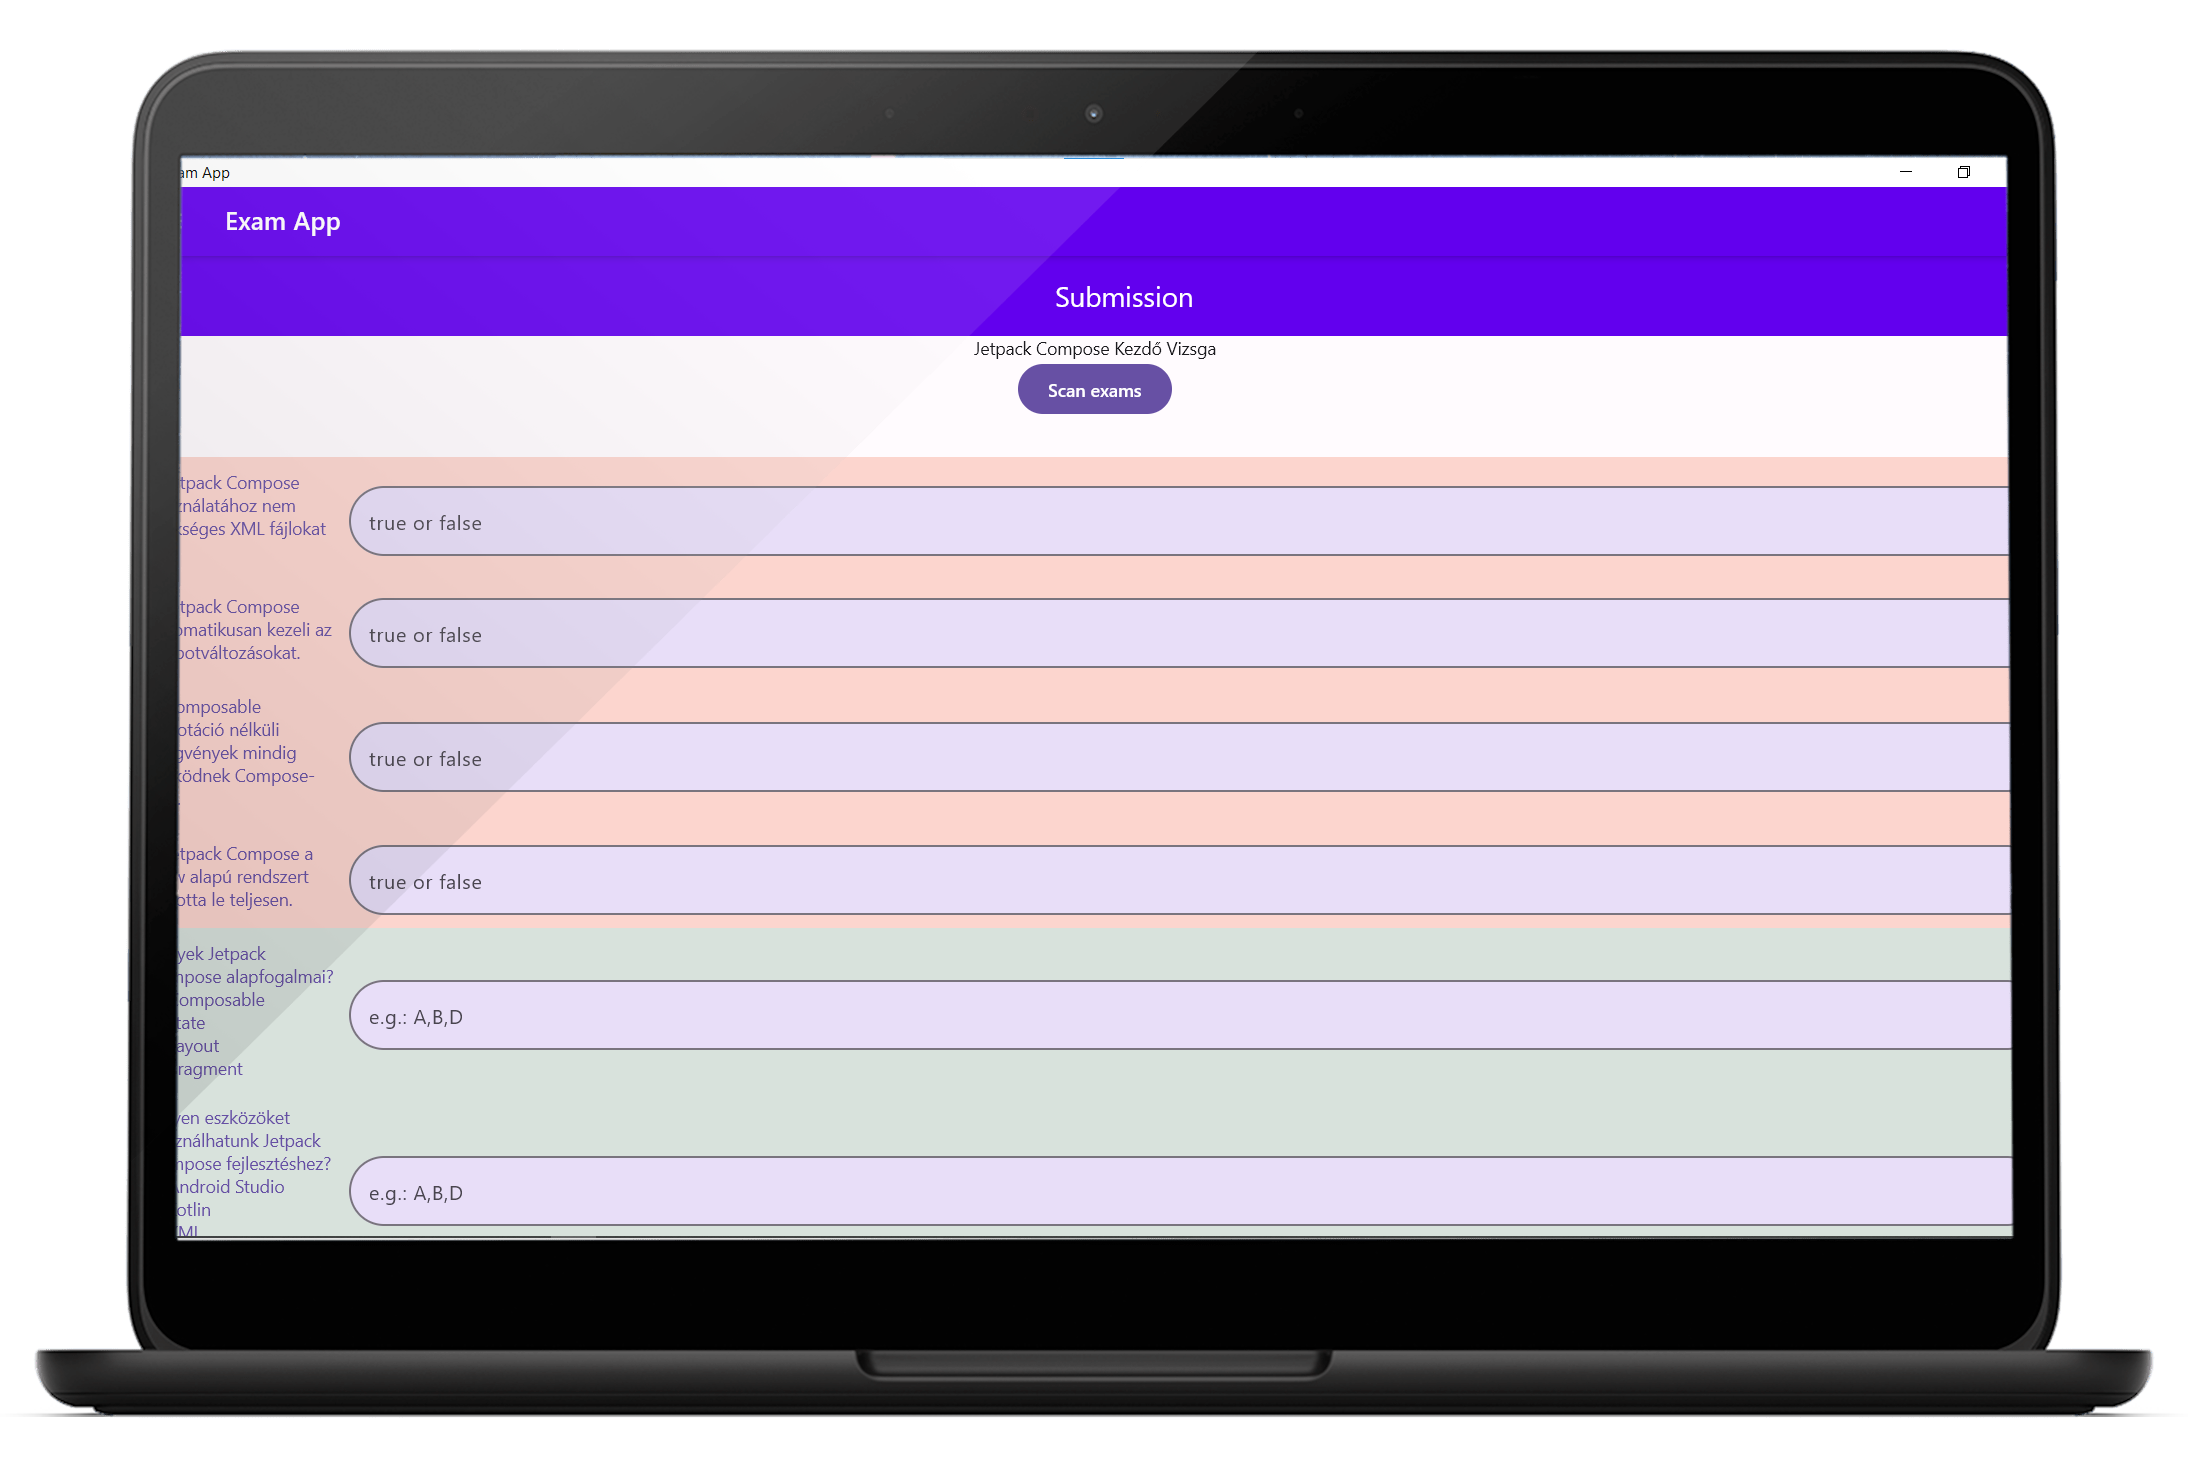
\includegraphics[width=0.6\textwidth, keepaspectratio]{figures/Submission_Desktop_framed.png}
    \end{tabular}
    \caption{Új feleletválasztós kérdés létrehozása.}
    \label{fig:SubmissionScreen}
\end{figure}


\subsection{Szekvencia diagram egy átlagos interakcióra}

Végezetül szeretnék bemutatni egy szekvencia diagramot, amin keresztül megérthető, hogy a felhasználó, az alkalmazás és a háttérben futó szerver milyen kapcsolatban állnak egymással.

\begin{figure}[!ht]
    \centering
    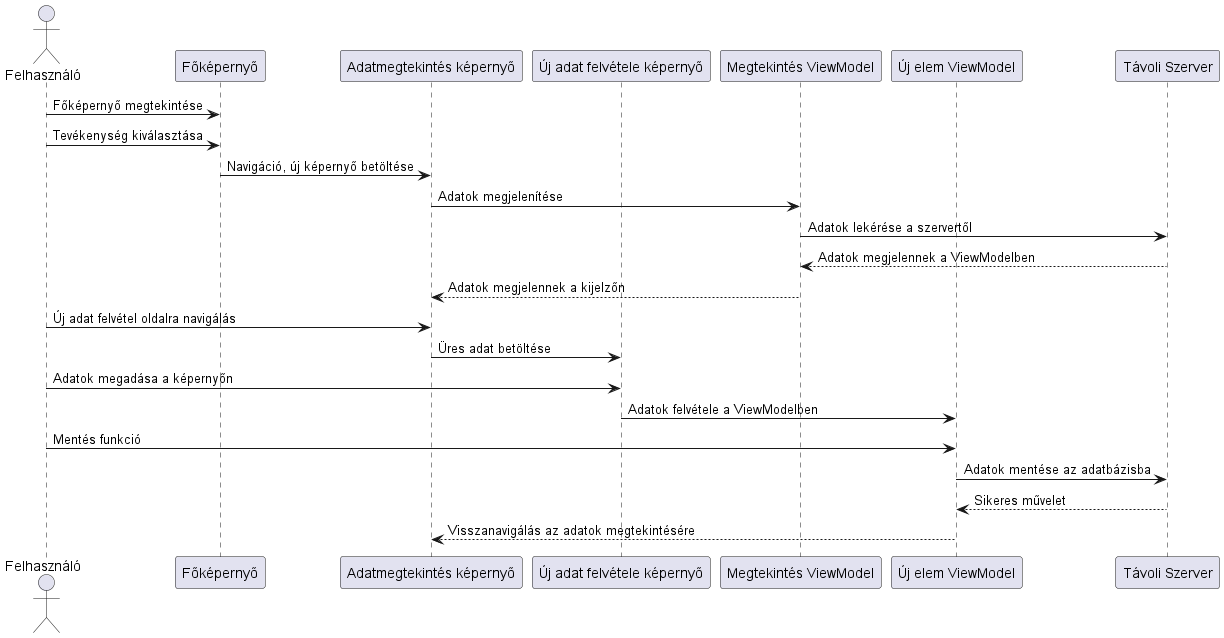
\includegraphics[width=150mm, keepaspectratio]{figures/Defaut Communication.png}
    \caption{Szekvencia diagram az end-to-end kommunikációról}
    \label{fig:DefaultCommunication}
\end{figure}

\section{Navigáció}
\label{sec:Nav}

A szoftverben az Android-ból jól ismert navigációs könyvtárat használtam.
Szerencsére már könnyen integrálható a multiplatform környezetekben.
A \refstruc{sec:Navigation}-ban erről már felületesen bemutattam.
Az ebben a fejezetben bemutatott implementációs lépéseket most részletesebben bemutatom.

Az első lépés kifejezetten egyszerű.
Létre kell hozni egy, a végpontokat összefogó sealed class-t, érdemes ennek egy route String típusú változót.
Ez leginkább a böngészőbeli routingra hasonlít.
A sealed class-ból leszármaztathatunk data object-eket. Ez egy viszonylag egyedi felhasználás.
Itt az object egy singleton minta, mivel ebből az osztályból egy példány keletkezik összesen a program futása során.
A data kulcsszó pedig létrehoz hasznos metódusokat az adateléréshez.
Tudunk megadni a leszármaztatott osztályokban egyéb paramétereket, így például tudunk egyes elemekre kulcsot adni, amit ennek felhasználásával tudjuk a konkrét példányt lekérdezni az adatbázisból.

\begin{lstlisting}[caption={Példa a végpontok felvételére.}, label={lst:NavDestExample}, language=Kotlin]
sealed class ExamDestination(val route: String) {
    data object LoginScreenDestination : ExamDestination("LoginScreen")

    data object TopicDetailsDestination : ExamDestination("TopicDetails") {
    const val topicIdArg = "0"
    val routeWithArgs = "$route/{$topicIdArg}"
    }
}        
\end{lstlisting}

A második lépésben a NavHostController-t kell létrehozni. Ezt a rememberNavController() meghívásával tudjuk megtenni egy Composable függvény törzse belül.
Ezt követően szükség lesz NavHost létrehozására, ami egy Composable függvény.
Ennek lehet átadni az előbb létrehozott NavHostController-t, és be kell állítani egy kezdeti végpontot, ami az első composition során fog megjelenni.

A lenti példakódban látható, hogy milyen módon lehet a NavHost-on belül felevenni és használni a végpontokat.
Számos paraméter megadható, de ezek közül csak a route kötelező.
Megadhatók egyéb argumentumok, amiket az egyik képernyőről a másiknak szeretnénk átadni navArgument-ek formájában.
Ezzel lehet például az egyedi azonosítókat átadni a lista nézetről a részletes nézetnek.
Ezt követően az utolsó kötelező elem megadása a content, aminek a típusa: @Composable AnimatedContentScope.(NavBackStackEntry).
Ebből két dolog következik: ez egy Composable scope, így hívhatunk Composable függvényeket innen, és hozzáférünk a backstackEntry-re tett adatokat, így például az argumentumokat.
Szintén ebben a lambda scope-ban hozzáférünk a navController-hez, amivel a navigációt megvalósító függvényeket tudjuk átadni a View-nak.

\begin{lstlisting}[caption={Példa egy végpont felvételére a navigációs gráfban.}, label={lst:NavEndPointExample}, language=Kotlin]
composable(
    route = ExamDestination.TopicDetailsDestination.routeWithArgs,
    arguments = listOf(navArgument(ExamDestination.TopicDetailsDestination.topicIdArg) {
        type = NavType.StringType
    })
) {
    val id = it.arguments?.getString(ExamDestination.TopicDetailsDestination.topicIdArg) ?: "0"
    TopicDetailsScreen(
        navigateToEditTopic = { navController.navigate("${ExamDestination.TopicEditDestination.route}/$id") },
        topicId = id,
        navigateBack = { navController.popBackStack() }
    )
}    
\end{lstlisting}

A viewban, azaz a Composable függvényben a \ref{lst:NavEndPointExample}.~kódrészletben megírt függvényt tudjuk meghívni.

\begin{lstlisting}[caption={A navigáció viewban való megjelenése.}, label={lst:NavView}, language=Kotlin]
fun TopicDetailsScreenUiState(
    navigateToEditPoint: (String) -> Unit,
    navigateBack: () -> Unit,
    ...
){
    Scaffold(
        topBar = { TopAppBarContent(stringResource(Res.string.topic_details), navigateBack) },
        floatingActionButton = {
            FloatingActionButton(
                onClick = { navigateToEditPoint(topic.uuid) },
                shape = MaterialTheme.shapes.medium,
                modifier = Modifier.padding(20.dp)

            ) {...}
        }
    ) { ... }
}

\end{lstlisting}

\section{ViewModel}
\label{sec:VM}

A ViewModel-lel korábban a \refstruc{sec:ViewModel} és a \refstruc{sec:HighLevelArchitecture} részekben már foglalkoztam vele.
Ebben a részben a megvalósításával fogok foglalkozni.

\begin{lstlisting}[caption={ViewModel implementációja.}, label={lst:VMImplementation}, language=Kotlin]
class TopicDetailsViewModel(
    var topicId: String,
) : ViewModel() {

    var topicDetailsScreenUiState: TopicDetailsScreenUiState by mutableStateOf(TopicDetailsScreenUiState.Loading)
    var uiState by mutableStateOf(TopicDetailsUiState())
    
    init { getTopic(topicId) }

    fun setId(id: String){ topicId = id; getTopic(id) }

    fun getTopic(topicId: String){
        topicDetailsScreenUiState = TopicDetailsScreenUiState.Loading
        viewModelScope.launch {
            topicDetailsScreenUiState = try{
                val result = ApiService.getTopic(topicId)
                uiState = TopicDetailsUiState(result.toTopicDetails(
                    parentName =
                    if (result.parentTopic == "null") ""
                    else ApiService.getTopic(result.parentTopic).topic
                ))
            TopicDetailsScreenUiState.Success(result)
            } catch (e: ApiException) {
                TopicDetailsScreenUiState.Error.errorMessage = e.message?: "Unkown error"
                TopicDetailsScreenUiState.Error
            }
        }
    }

    suspend fun deleteTopic() {
        try { ApiService.deleteTopic(topicId)} 
        catch (e: ApiException) {
            TopicDetailsScreenUiState.Error.errorMessage = e.message?: "Unkown error"
            topicDetailsScreenUiState = TopicDetailsScreenUiState.Error
        }
    }
}
\end{lstlisting}

A \ref{lst:VMImplementation}.~kódrészleten keresztül bemutatom a legfontosabb elemeket.
A ViewModel osztály az általános Android ViewModel osztályból származik le.
Ez teszi lehetővé többek között a ViewModelScope használatát.
A szokásos módon adhatunk paramétereket, ebben az esetben így adjuk át az ID-t, amivel a REST API-n keresztül tudjuk elérni a kívánt témakört.

Érdemes az osztály elején felvenni az állapotokat.
Ilyen Statekben tárolom a képernyő állapotát és a képernyőn megjelenő adatokat is.
Ezeket a megfelelő kezdőértékkel létrehozva használhatjuk őket.
Lehetne MutableStateFlow is, de immutábilis State-et használni egy másik megoldásként.

Az init{} blokk egyszer hívódik meg, az objektum létrehozása során, a konstruktor után. Ebből lehet több blokk is, amik a leírt sorrendben hívódnak meg. Későbbi init blokkban használhatjuk a korábbi értékeket.
Most itt egy aszinkron művelet eredményeként kapjuk meg az adatot.
Ezen kívül egy másik inicializációs elem a setId függvény, erre akkor van szükség, amikor egy specifikus elemet akarunk megjeleníteni.

Az init{} blokkban nem tudunk tényleges aszinkron függvényeket hívni, ezért szükséges a töltőképernyő, amíg az adatok megérkeznek.
A getTopic függvény kezeli le ezt a részt. Első lépés a töltőképernyő beállítása. Ezt követően kihasználjuk a viewModelScope-ot, ahol végrehajthatunk hosszabb műveletet anélkül, hogy a UI szál lefagyjon addig.
Itt megvárjuk, amíg a REST API visszaküldi az adatokat, siker esetén a Success képernyőt állítjuk be a state-ben, hiba esetén erről adunk tájékoztatást.

Egyéb függvények megadhatók aszinkron módon, mint a törlés például, ezt nem kell megvárnunk.

\section{HTTP kliens}
\label{sec:HTTP}

Ebben a részben a HTTP-kliens működését mutatom be.

\begin{lstlisting}[caption={HTTP kliens.}, label={lst:HTTPClient}, language=Kotlin]
object ApiService {
    private val httpClient = HttpClient() {
        install(ContentNegotiation) {
            json(Json {
                ignoreUnknownKeys = true
                prettyPrint = true
            })
        }
        defaultRequest { url("http://mlaci.sch.bme.hu:46258")  /* Set the base URL */ }
    }
    
    suspend fun getPoint(id: String): PointDto {
        val response = httpClient.get("/point/$id")
        if (response.status == HttpStatusCode.OK) return response.body()
        throw ApiException(handleHttpException(response.status))
    }

    suspend fun postPoint(point: PointDto): PointDto? {
        val response = httpClient.post("/point") {
            contentType(ContentType.Application.Json)
            setBody(point)
        }
        if (response.status == HttpStatusCode.Created) return response.body()
        throw ApiException(handleHttpException(response.status))
    }
}
\end{lstlisting}


A \ref{lst:HTTPClient}.~kódrészletben egy kis rész látható a kommunikáció működéséről.
Egy objektumban valósítom meg, így csak egy példány készül belőle.
Létrehozok benne egy HttpClientet, aminek beállítom a tartalom típusát JSON-ra, és az alapértelmezett URL is beállításra kerül. 
Az endpointokban megadott részek ehhez lesznek hozzáfűzve, így kevesebb kódot kell írni, és kevesebb hibázási lehetőség van.

Ezek alatt aszinkron, suspend függvények találhatóak. Mind a GET, POST, PUT és DELETE műveletekre vannak, de a GET-en és a POST-on keresztül a lényeges részeket be lehet mutatni.
A függvények kaphatnak paramétereket, a GET esetén egy stringet, ami a UUID értékét tartalmazza.
A visszatérési értéke pedig egy adott típusú DTO lesz.
A kérést a baseURL + megadott útvonalra továbbítja a Ktor. Ezt a stringet lehet paraméterezni is, például az id-val.
A válaszban megkapjuk a státuszkódot, és a válasz törzsében siker esetén a kért objektumot, amit a KotlinX szerializáció állít elő a JSON adatból, amit ténylegesen kapunk.
Hiba esetén a felhasználónak adunk erről visszajelzést egy saját kivételosztály segítségével, 200 OK válasz esetén pedig átadjuk az elkészült adatot.
A listázás és a törlés ehhez hasonló módon történik.

Az alsó függvény az új adat létrehozását mutatja be, lényegében a módosítás is szinte pont így történik, csak ott a PUT metódust kell hívni, és a Created státuszkódot várjuk helyes visszatérés esetén.
Itt paraméternek az objektumot kapjuk, amit a POST üzenet törzsében állítunk be. Itt történik meg a JSON szerializáció, de most sem kell ezzel külön foglalkozni, elég, ha az adattípusát megadjuk.
Innentől minden ugyanúgy történik, mint a többi esetben.

\section{PDF exportáló funkció}
\label{sec:PDF}

A feladatsor PDF-be exportálása más módon zajlik a két platformon. 
Alapvetően hasonlóan működnek.
Be kell állítani a megfelelő betűtípusokat, oldalméreteket, szövegméretet és hasonló egyéb változókat.

Ezt követően float típusú értékek segítségével lehet pozícionálni a kiírandó szövegeket.
Táblázatokat nem lehet rajzolni, de egyéb geometriai elemeket, így vonalat igen, ezekből elkészíthető egy táblázat is.
Csak alacsony szintű támogatása van az API-knak, így ugyan minden elkészíthető, de nagyon időigényes.
Ahhoz, hogy egy jól kinéző dokumentum készüljön, nagyon sok időt kell beletenni a megvalósításba.
PDF szerkesztésére és létrehozására így tehát nem ezek a legjobb megoldások.

\section{Szöveg felismerés}
\label{sec:TextRec}

A Szövegfelismeréshez a Google ML-Kit megoldását választottam.
Sok előre elkészített, egyszerű AI modellt tartalmaz, amit könnyen lehet a kódban hasznosítani.
A használatát a \ref{lst:TextRec}.~kódrészlet mutatja be. 
A teljes kód látható egyben, mivel tömören és hatékonyan megoldható a probléma.
Ez a funkció Android eszközökön támogatott, asztali eszközökön nagyon furcsa lenne a használata.

Az osztály örökli az ImageAnalysis.Analyzer-t, így lehet képeket feldolgozó kódot létrehozni.
Be kell állítani az alapértékeket, amikkel majd tud dolgozni az AI.
Ezt követően meg kell írni az egyetlen függvényt, amit felülírni kell, itt történik a kép feldolgozása, paramétere egy ImageProxy.
A szükséges hibakezelés után egy háttérszálon végrehajtódik a szöveg megkeresése és felismerése a képen.
A szöveget ezt követően átadja a kód egy másik függvénynek, amit paraméterben adtunk meg, így tudjuk kinyerni az értékes adatokat.
Ez a kód, amíg az adott nézeten vagyunk, végtelen ideig fut, ezért szükség van egy kis késleltetésre, ezzel elkerülve a felesleges hardver használatot.

\begin{lstlisting}[caption={Szövegfelismerés.}, label={lst:TextRec}, language=Kotlin]
actual class TextRecognitionAnalyzer actual constructor(
    private val onDetectedTextUpdated: (String) -> Unit
) : ImageAnalysis.Analyzer {

    actual companion object {
        const val THROTTLE_TIMEOUT_MS = 1_000L
    }

    private val scope: CoroutineScope = CoroutineScope(Dispatchers.IO + SupervisorJob())
    private val textRecognizer: TextRecognizer =
        TextRecognition.getClient(TextRecognizerOptions.DEFAULT_OPTIONS)

    @OptIn(ExperimentalGetImage::class)
    override fun analyze(imageProxy: ImageProxy) {
        scope.launch {
            val mediaImage: Image = imageProxy.image ?: run { imageProxy.close(); return@launch }
            val inputImage: InputImage =
                InputImage.fromMediaImage(mediaImage, imageProxy.imageInfo.rotationDegrees)

            suspendCoroutine { continuation ->
                textRecognizer.process(inputImage)
                    .addOnSuccessListener { visionText: Text ->
                        val detectedText: String = visionText.text
                        if (detectedText.isNotBlank()) {
                            onDetectedTextUpdated(detectedText)
                        }
                    }
                    .addOnCompleteListener {
                        continuation.resume(Unit)
                    }
            }

            delay(THROTTLE_TIMEOUT_MS)
        }.invokeOnCompletion { exception ->
            exception?.printStackTrace()
            imageProxy.close()
        }
    }
}
\end{lstlisting}